\documentclass[10pt,a4paper]{article}
\usepackage[margin=2.0cm]{geometry}
\usepackage{amsmath,amssymb}
\usepackage{graphicx}
\usepackage{booktabs}
\usepackage{longtable}
\usepackage{float}
\usepackage{array}
\usepackage{xcolor}
\usepackage[font=small,labelfont=bf]{caption}
\usepackage{microtype}
\usepackage{enumitem}
\usepackage[hidelinks]{hyperref}

\definecolor{tmblue}{HTML}{2A78D6}
\definecolor{frorange}{HTML}{EB6834}
\definecolor{fraqua}{HTML}{1BAF7A}
\definecolor{ink2}{HTML}{52514E}
\definecolor{boxfill}{HTML}{EEF4FC}
\definecolor{warnfill}{HTML}{FDF0EA}

\setlist{itemsep=2pt,topsep=3pt}
\setlength{\LTleft}{0pt}
\setlength{\LTright}{0pt}
\setlength{\LTcapwidth}{\linewidth}
\captionsetup[longtable]{width=\linewidth}
\renewcommand{\arraystretch}{1.12}
\emergencystretch=2em
\graphicspath{{m11-gui/}}

% \input inside a tabular puts a \relax before the next \bottomrule ("Misplaced \noalign"): use the primitive.
\makeatletter\newcommand{\tabinput}[1]{\@@input #1 }\makeatother
\newcommand{\code}[1]{\texttt{#1}}
\newcommand{\notmet}{\textcolor{frorange}{\textbf{not met}}}
\newcommand{\met}{\textcolor{fraqua}{\textbf{met}}}

\title{\textbf{TraceMaker}\\[2pt]\large Roadmap and test report\\[2pt]
\normalsize Every milestone, every test, every benchmark run, as of the close of the roadmap}
\author{Development report}
\date{6 October 2026}

\begin{document}
\maketitle

\begin{abstract}
\noindent This report records the state of the TraceMaker roadmap (milestones M0 to M13) and everything that was
done to test the software: the test suite test by test, the build presets it runs under, the benchmark sets and
the judge, every benchmark run on record, the held-out sets built for the placement gate, and each experiment of
the close-out with its configuration and result. All fourteen milestones are closed: every task is either built
and measured or closed with the measurement that shows why it was not built. Closed does not mean every gate is
met. Two gates are not met (M8: from-scratch placement gives 85\,\% clean boards against a gate of 90\,\%; M9: 41\,\%
of the dense-package boards are clean) and one comparison was never measured (M7 against the SA-PCB placer). The
test suite has 132 tests and passes in the release and CPU-only builds; the address-sanitizer build reports no
memory error. On the main routing benchmark the final binary routes 100, 70.0, 63.3 and 54.5\,\% of the sampled
boards of tiers A to D with no error added by routing, against 100, 50.0, 46.7 and 36.4\,\% published for
Freerouting 2.5.
\end{abstract}

\tableofcontents
\newpage

% ------------------------------------------------------------------------------------------------------------
\section{How to read this report}

The tables in Sections~\ref{sec:roadmapdetail}, \ref{sec:alltests}, \ref{sec:perboard} and \ref{sec:allruns}, and
the summary tables that carry counts, are generated by \code{report/make\_test\_report.py} from the project's own
records: \code{dev/progress.json} (the roadmap), the JUnit file of a full test run, the test sources, and
\code{bench/results/*/summary.json} with their per-board files. A number in those tables is the number in the
record. The text sections were written by hand from the design documents (\code{docs/}), the decision log
(\code{docs/12-decisions.md}, D1 to D64) and the experiment logs; each experiment names the files that hold its
raw results.

Three words are used with fixed meanings throughout.
\begin{description}[leftmargin=1.2em,itemsep=2pt]
\item[Clean.] A routed board is clean when KiCad's own design-rule check reports no unconnected item and no
  error that the run added (Section~\ref{sec:judge}).
\item[Closed.] A roadmap task is closed when it is built and measured, or when a measurement shows that building it
  would not help and it is recorded as not built with that measurement.
\item[Gate.] The test or benchmark result a milestone was meant to reach. A closed milestone can have an unmet
  gate; Table~\ref{tab:gates} says which.
\end{description}

% ------------------------------------------------------------------------------------------------------------
\section{Roadmap summary}

\begin{table}[H]
\centering\small
\begin{tabular}{@{}llrrrl@{}}
\toprule
 & Milestone & Tasks & Built & Closed unbuilt & Gate \\
\midrule
\tabinput{generated/roadmap_summary.tex}
\bottomrule
\end{tabular}
\caption{The fourteen milestones. ``Built'' counts tasks that were implemented and measured; ``closed unbuilt''
counts tasks closed with a measurement instead of an implementation. The gate column is ``met'' when the progress
record carries no dissenting gate result.}
\label{tab:roadmap}
\end{table}

\begin{table}[H]
\centering\small
\begin{tabular}{@{}lp{0.37\linewidth}p{0.50\linewidth}@{}}
\toprule
 & Gate & Result \\
\midrule
M0 & CPU and CUDA tests on both GPUs; \code{kicad-cli} works from the harness & \met \\
M1 & Byte-identical round trip of every fixture board; netlist equals KiCad's & \met \\
M2 & Same violations as \code{kicad-cli pcb drc} on all fixture boards & 14 of 17 demo boards exact, 264 of 264 injected-defect boards; three boards differ in documented ways \\
M3 & Viewer at 60 frames per second; replay reproduces the board & replay \met; frame rate not measured (no GPU-backed browser on the machine) \\
M4 & Simple set routed with zero added KiCad errors & \met \\
M5 & Completion at least Freerouting's on its test set & \met\ (tier A: 100\,\% clean, equal to Freerouting 2.5) \\
M6 & CPU and GPU identical; time to route reduced on dense boards & \met\ for the GPU workload in use (cost-to-go fields); global routing did not contribute \\
M7 & Legal placements; wirelength at most SA-PCB's & legality \met; the SA-PCB comparison was \textbf{not measured} (the baseline does not build without SWIG) \\
M8 & From-scratch clean pass at least 90\,\%; \code{eco} closes boards & \notmet: 85\,\% (34 of 40 held-out boards) \\
M9 & BGA boards complete & \notmet: 41\,\% of 17 dense-package boards clean (Freerouting 2.5: 24\,\%) \\
M10 & Bit-identical across thread counts and GPU on/off & \met \\
M11 & Round trip in KiCad on the demo boards & \met, in a running KiCad 10.0.6 GUI driven without a desktop \\
M12 & Each feature gated by its own subset; no regressions & \met\ per feature (Section~\ref{sec:experiments}) \\
M13 & Detection precision and recall; every applied rule met or reported; no regression & \met \\
\bottomrule
\end{tabular}
\caption{Gates and their results.}
\label{tab:gates}
\end{table}

% ------------------------------------------------------------------------------------------------------------
\section{How TraceMaker is tested}

\subsection{The judge}\label{sec:judge}

Every routing and placement result is judged by KiCad itself, not by TraceMaker's own checker:
\code{kicad-cli pcb drc --severity-all --all-track-errors} from the Docker image \code{kicad/kicad:10.0.6}, run on
the input board and on the output board (\code{bench/run.py}, function \code{drc}).
\begin{itemize}
\item \textbf{Added routing errors} are the violations of severity \emph{error} that involve a track, an arc or a
  via, counted by type, output minus input. Types that routing cannot cause (silkscreen, courtyards, library
  mismatches, unconnected items, dangling tracks) are excluded from this count; unconnected items are counted
  separately.
\item \textbf{Added placement errors} (when TraceMaker moved parts) are courtyard overlaps, holes inside
  courtyards, copper-to-edge and copper clearance, shorts, solder-mask bridges and hole clearances between
  different footprints, placed board minus the designer's board.
\item A board is \textbf{clean} when KiCad lists no unconnected item on the output and both counts above are
  empty.
\item \textbf{Completion} is one minus unconnected items after over unconnected items before.
\end{itemize}
PCBench boards come without their project files, so KiCad's default rules apply (track 0.25\,mm, clearance
0.2\,mm, via 0.8/0.4\,mm). Section~\ref{sec:humanbaseline} shows what that does to the benchmark: only 6 of 92
designer-routed boards pass the same judge.

\subsection{Environment}

\begin{table}[H]
\centering\small
\begin{tabular}{@{}ll@{}}
\toprule
Machine & 56 cores, about 150\,GB RAM, Tesla P100 (12\,GB) and Tesla V100 (16\,GB), shared with other jobs \\
Compilers & GCC 15 for C++20; CUDA 12.4 with \code{g++-13} as host compiler \\
Warnings & \code{-Wall -Wextra -Wpedantic -Wshadow -Wconversion} and more, with \code{-Werror} \\
KiCad & 10.0.6 from Docker (\code{kicad-cli}, and \code{pcbnew} for the GUI test) \\
Freerouting & published PCBench results for 2.5.0-RC12 and 2.4.1; 2.5.0-RC12 and 1.9.0 run locally for the quality study \\
Test framework & Catch2 3 through CTest, JUnit results per test \\
\bottomrule
\end{tabular}
\caption{Test environment.}
\end{table}

\noindent Four build presets are tested. \code{release} is the one benchmarks use. \code{cpu-only} builds without
CUDA and proves that everything works with no GPU (GPU tests skip). \code{asan} adds the address and
undefined-behaviour sanitizers. \code{tsan} (thread sanitizer) exists as a preset and was not run in the
close-out.

\subsection{Levels of testing}

\begin{enumerate}
\item \textbf{Unit tests} (Catch2, 116 test cases in 15 source files): geometry predicates, the s-expression
  parser and writer, the KiCad reader, rule reading, the random-number generator, the placer's parts, the
  component-rule catalogue and detection, impedance formulas against textbook and KiCad values, the event server
  and the replay log.
\item \textbf{Reference-path equivalence} (non-negotiable rule 3 of the project): every accelerated path has a
  plain reference path and a test that both give the same result. Table~\ref{tab:equiv} lists them.
\item \textbf{Integration tests} (16, scripts under \code{tests/integration}): they run the real binaries on real
  boards and compare with KiCad, with a second run, or with the reference path.
\item \textbf{Benchmarks} judged by KiCad on PCBench tiers A to D, the dense-package set, DAC 2020, and a
  held-out quality study against Freerouting run on the same machine.
\item \textbf{Held-out sets} for placement: H (40 boards never used before) and S (the same boards with their parts
  piled), built for the M8 gate (Section~\ref{sec:held}).
\item \textbf{A running KiCad}: the plugin against \code{pcbnew} under a virtual display
  (Section~\ref{sec:gui}).
\end{enumerate}

\begin{table}[H]
\centering\small
\begin{tabular}{@{}p{0.27\linewidth}p{0.27\linewidth}p{0.38\linewidth}@{}}
\toprule
Accelerated path & Reference path & Test \\
\midrule
GPU Philox random fill & CPU fill & bit-identical on every device (\code{test\_gpu.cpp}) \\
GPU cost-to-go fields (CUDA sweeps) & CPU sweeps & equal on random grids (\code{test\_gpu.cpp}); routing identical with and without GPU (\code{thread\_determinism}) \\
Zone-fill edge index for the DRC & every edge of every fill (\code{drc --linear-zones}) & \code{[geom]} equivalence test on random shapes; \code{drc\_zone\_index} on four boards; vme-wren and jetson compared by hand, byte-identical \\
Polygon index for disks & \code{closer\_than} & \code{[geom]} test, 4,000 disks \\
Flood-fill reachability pre-check & full A* & \code{reach\_verify}: every ``unreachable'' re-checked, zero mismatches \\
Incremental routability term in the annealer & from-scratch recompute & placer unit test \\
Portfolio on a thread pool & one thread & \code{thread\_determinism}: identical bytes at 1, 3 and 8 threads \\
Placer's translated closeness test & \code{geom::closer\_than} & placer unit test \\
Exact windows by branch and bound & full enumeration & placer unit test \\
Python module & command-line binary & \code{python\_bindings}: identical boards \\
Recording and live view & plain routing & \code{record\_replay}: identical boards \\
\bottomrule
\end{tabular}
\caption{Accelerated paths, their reference paths and the tests that hold them equal.}
\label{tab:equiv}
\end{table}

\subsection{Determinism as a test method}

The router has two budgets. \code{--time} is a wall-clock limit and makes results depend on machine load.
\code{--work} is a budget in search expansions: the same input, seed and budget give the same bytes at any
thread count and with or without a GPU (decision D47). Every experiment in Section~\ref{sec:experiments} was first
measured with \code{--work} (one variant or all eight), where a difference of one connection is real, and only
then on the KiCad-judged tiers at 120 seconds, where the eight-variant portfolio and machine load add noise. Two
results in this report show why both are needed: a planning change that routed 81 more connections at a fixed
budget was neutral on the tiers, and a tier run made while two others were running read 52 connections lower
than the same binary side by side with its control.

\subsection{Rules for experiments}

\begin{itemize}
\item Compare two configurations of the \emph{same binary}, run at the same time on the same machine.
\item Report losses and null results with the same weight as gains; a change that does not help is removed or
  left off, and the decision log says so.
\item Never tune on held-out boards. Sets H and S were built from boards that appear in no earlier result, list,
  test or document.
\item The quick tier (A) is run before a change to routing or placement is finished.
\end{itemize}

% ------------------------------------------------------------------------------------------------------------
\section{The test suite}

\subsection{Summary by source file}

\begin{table}[H]
\centering\small
\begin{tabular}{@{}p{0.48\linewidth}rrrrr@{}}
\toprule
Source & Tests & Passed & Skipped & Failed & Time (s) \\
\midrule
\tabinput{generated/tests_summary.tex}
\bottomrule
\end{tabular}
\caption{Release build, full run at the end of the close-out. Appendix~\ref{sec:alltests} lists every test.}
\label{tab:testsummary}
\end{table}

\subsection{Results by build preset}

\begin{table}[H]
\centering\small
\begin{tabular}{@{}lp{0.74\linewidth}@{}}
\toprule
Preset & Result at the end of the close-out \\
\midrule
\code{release} & 132 of 132 pass (303 to 440 seconds depending on load). \\
\code{cpu-only} & 132 of 132: 130 pass, the two GPU equivalence tests skip as designed. \\
\code{asan} & No sanitizer report in any test. Unit tests pass. The slow integration tests were rerun one at a
  time on an idle machine after their limits were adjusted (below) and pass: \code{drc\_zone\_index} 546\,s,
  \code{global\_route} 526\,s, \code{diff\_pair} 891\,s, \code{thread\_determinism} 1,163\,s, \code{crules\_two\_stage}
  1,654\,s. The preset was not rerun end to end afterwards. \\
\code{tsan} & Not run in the close-out. \\
\bottomrule
\end{tabular}
\caption{Test results per preset.}
\end{table}

\paragraph{What the sanitizer run exposed in the tests themselves.} On a fully loaded machine four integration
tests ran into their time limits under \code{asan} and \code{diff\_pair} failed with 111 of 113 connections
routed. None was a memory error. \code{diff\_pair} set a work budget but left the router's default 120-second
wall clock in force, so a slow build stopped early; it now passes \code{--time 3600}, which makes the work budget
the only limit. \code{crules\_two\_stage} anneals at a fifth of the default effort (it checks legality and
locking, not quality). The two tests added in the close-out were made lighter (four boards instead of six; a
3\,M instead of an 8\,M budget), and the limits of the slow tests were raised to 30 and 60 minutes.

\subsection{What the integration tests check}

Appendix~\ref{sec:alltests} carries a one-line description under each of the sixteen integration tests. The three
that compare with KiCad carry the most weight:
\begin{itemize}
\item \code{kicad\_drc\_parity}: TraceMaker's DRC against KiCad's on 14 demo boards, violation types equal.
\item \code{kicad\_drc\_broken\_parity}: 264 boards with injected defects, equal violation by violation.
\item \code{kicad\_edit\_roundtrip}: boards written by TraceMaker read back identically in pcbnew.
\end{itemize}
Untouched content of a \code{.kicad\_pcb} file round-trips byte for byte (rule 8); that is tested on the fixture
boards in \code{test\_kicad\_io.cpp}.

% ------------------------------------------------------------------------------------------------------------
\section{Routing benchmarks}

\subsection{Sets}

\begin{table}[H]
\centering\small
\begin{tabular}{@{}lp{0.20\linewidth}rp{0.48\linewidth}@{}}
\toprule
Set & Source & Boards & Use \\
\midrule
PCBench tier A & Freerouting's benchmark fixtures & 40 & quick tier: run before any routing change is finished \\
PCBench tier B & same & 40 & main comparison with Freerouting's published results \\
PCBench tier C & same & 30 & same \\
PCBench tier D & same & 22 & largest boards (600 to 1,600 connections) \\
Dense-package set & PCBench boards with BGAs and fine-pitch parts & 17 & escape planning (M9) \\
Quality study & 60 PCBench boards unused in development & 60 & Freerouting 2.5.0-RC12 and 1.9.0 run locally, same judge \\
Hard set & 10 to 24 large and nearly clean boards & 24 & fixed-budget experiments (\code{bench/m6\_bench.py}) \\
KiCad demos & KiCad 10 & 17 & DRC parity, rule coverage, the GUI test \\
DAC 2020 & hand-routed boards & 11 & vias and layers against human routing \\
H / S & held-out, built 2026-10-06 & 40 & placement gate (Section~\ref{sec:held}) \\
\bottomrule
\end{tabular}
\caption{Benchmark sets. Tier samples are seeded and fixed; the same boards are used in every tier run.}
\end{table}

\subsection{Final result}

All tier runs use eight router variants on eight threads, 120 seconds per board, and KiCad's DRC as judge.
Table~\ref{tab:final} compares the binary at the start of the close-out with the final one. The final four
tiers were run at the same time (64 router threads on 56 cores), so their routed totals are a little low; the
clean-pass counts are what the table is for.

\begin{table}[H]
\centering\small
\begin{tabular}{@{}lrrrrrr@{}}
\toprule
 & \multicolumn{2}{c}{Start of close-out (\code{reach1})} & \multicolumn{2}{c}{Final (\code{final11})} & Freerouting & Boards with \\
Tier & Clean & Routed & Clean & Routed & 2.5 clean & added errors \\
\midrule
A (40 boards) & 100\,\% & 2,637 & 100\,\% (40) & 2,637 & 100\,\% & 0 \\
B (40) & 67.5\,\% & 5,165 & 70.0\,\% (28) & 5,172 & 50.0\,\% & 0 \\
C (30) & 63.3\,\% & 9,523 & 63.3\,\% (19) & 9,516 & 46.7\,\% & 0 \\
D (22) & 50.0\,\% & 16,628 & 54.5\,\% (12) & 16,522 & 36.4\,\% & 0 \\
\bottomrule
\end{tabular}
\caption{Clean pass and connections routed. Tier D's twelfth clean board (m2fc) closes its last connection or not
from run to run; side by side earlier the same day tier D read 16,618 and 16,622 routed with 12 clean both ways.
Tier B's gain is one board from the half-pitch variant (Section~\ref{sec:experiments}).}
\label{tab:final}
\end{table}

Appendix~\ref{sec:perboard} lists every board of the final runs; Appendix~\ref{sec:allruns} lists every benchmark
run on record since the project began.

\subsection{What the benchmark measures, and what it cannot}\label{sec:humanbaseline}

Three studies in the close-out examined the benchmark itself.

\paragraph{The designers' own layouts under the same judge} (\code{bench/human\_baseline.py}; the routed
\code{raw.kicad\_pcb} of the 92 boards of tiers B to D).

\begin{table}[H]
\centering\small
\begin{tabular}{@{}p{0.66\linewidth}r@{}}
\toprule
Designer's layout clean & 6 of 92 \\
TraceMaker non-clean boards whose designer's layout is not clean either & 33 of 34 \\
TraceMaker clean boards whose designer's layout has errors on routed copper & 52 of 58 (median 108 errors) \\
Designer used copper zones that the unrouted fixture no longer has & 82 of 92 \\
Open connections on non-clean boards that are on a net the designer poured & 32 of 938 \\
\bottomrule
\end{tabular}
\caption{The benchmark is judged under rules that the original designs mostly do not meet.}
\end{table}

\paragraph{What if the poured nets were left to a pour.} The 34 non-clean boards were routed twice at the same
fixed budget (eight variants, 60\,M expansions): with all nets, and with the designer's zone nets skipped. Four
boards complete without them; open connections fall from 938 to 723. Missing pours contribute on a few boards and
are not the main cause.

\paragraph{Why the last connections fail.} After a reporting fault was fixed (Section~\ref{sec:faults}), nine
nearly clean boards were examined: on five, the last one to five connections are lost to nets that keep ripping
each other at one package; one board has pins sealed by fixed copper; two are boxed in before negotiation. On
serial\_gw the geometry is visible: a QFN at 0.5\,mm pitch whose centre pad has no net, pins 3 to 6 alternating
ground and supply, and no room for the vias the crossing needs under the default rules.

% ------------------------------------------------------------------------------------------------------------
\section{Held-out placement sets and the M8 gate}\label{sec:held}

\paragraph{Set H} (\code{bench/place\_sets/H.txt}, built by \code{bench/make\_place\_sets.py}, frozen). A seeded
sample (seed 7) of PCBench boards that appear in no earlier result, development list, test or document (342 boards
excluded), with 10 to 300 parts and at least 10 movable, a courtyard on at least 80\,\% of the parts, and routed
completely in the designer's placement in 120 seconds. Twenty boards at or below the candidates' median of 33
parts and twenty above: 14 to 138 parts, 4,022 connections; 132 candidates were tried.

\paragraph{Set S.} The H boards with every part that full-mode placement may move piled at the centre of the
board, so the file no longer contains the designer's placement. Parts the placer holds in the designer's board
(locked parts, edge connectors, mounting holes, parts overhanging the edge) stay, since a schematic does not say
where a connector goes.

\begin{table}[H]
\centering\small
\begin{tabular}{@{}p{0.50\linewidth}rr@{}}
\toprule
Run & Clean & Routed \\
\midrule
H, designer's placement, before the two router fixes (\code{H-none-1}) & 38 of 40 & 4,021 of 4,022 \\
H, designer's placement, after the Margin fix (\code{H-none-2}) & 38 of 40 & 4,019 of 4,022 \\
S, \code{full} mode as the placer was (\code{S-full-1}) & 28 of 40 (70\,\%) & 3,900 of 4,002 \\
S, \code{full --scratch} on the 12 failing boards (\code{S-full-4}) & 3 of 12 & \\
S, \code{routable --scratch}, first version (\code{S-routable-5}) & 33 of 40 (82.5\,\%) & 3,944 of 4,022 \\
S, \code{routable --scratch}, final (\code{S-routable-7}) & \textbf{34 of 40 (85\,\%)} & 3,939 of 4,013 \\
\bottomrule
\end{tabular}
\caption{The M8 gate asks for 90\,\%. It is not met.}
\end{table}

\noindent The six boards that fail in the final run: three have a part that fits nowhere without breaking copper,
hole or mask rules that the designer's placement itself breaks (an Arduino module; a 15\,mm IC between two pin
headers 12.4\,mm apart; a battery holder); kitspace\_hack cannot be routed clean in the designer's placement
either once Margin lines count as edges (89 of 92); ottawa-badges-2016 and pico-pi are three connections short
each. Of the 36 boards that can be clean, 34 are. More spacing between parts was tried on the two near misses
(courtyard clearance 0.6 and 1.0\,mm) and routed fewer connections (211 and 191 of 219 on pico-pi). Placement
takes 91 seconds at the median in \code{routable} mode. Table~\ref{tab:heldboards} gives every board.

{\footnotesize
\begin{longtable}{@{}p{0.33\linewidth}rrp{0.20\linewidth}p{0.24\linewidth}r@{}}
\caption{Held-out boards: the designer's placement (H) and from-scratch placement (S, final run). ``pl.\ err.''
are KiCad errors added by placement.}\label{tab:heldboards}\\
\toprule Board & Parts & Movable & H: routed, judged & S: routed, judged & Place (s) \\ \midrule \endhead
\tabinput{generated/held.tex}
\bottomrule
\end{longtable}
}

% ------------------------------------------------------------------------------------------------------------
\section{KiCad in the loop without a desktop}\label{sec:gui}

KiCad 10's programming interface only works against a running \code{pcbnew}. The script
\code{scripts/kicad\_gui\_roundtrip.py} starts a virtual display (Xvfb), runs \code{pcbnew} from the Docker image
on it with the API server enabled, dismisses KiCad's first-run wizard by synthetic mouse clicks, and then drives
TraceMaker's plugin against the live board through the API socket. It checks, in order:

\begin{table}[H]
\centering\small
\begin{tabular}{@{}p{0.50\linewidth}p{0.44\linewidth}@{}}
\toprule
Check & Result on \code{multichannel\_mixer-unrouted} \\
\midrule
KiCad starts and opens its API socket & yes \\
The API answers after the wizard is dismissed & yes (KiCad 10.0.6) \\
The plugin runs against the live board & 80 connections in 30 seconds \\
Copper appears in the open board & tracks 140 $\to$ 316, vias 19 $\to$ 21 \\
One undo removes the whole result & 140 tracks, 19 vias \\
Redo brings it back & 316 tracks, 21 vias \\
KiCad's DRC of the board saved from the GUI & unconnected 148 $\to$ 65, no new errors \\
\midrule
With placement (\code{--place refine}) & 65 footprints moved; old copper routed again; zones refilled \\
Two undos (zone refill, then the commit) restore everything & 140 tracks, 19 vias, footprints back \\
KiCad's DRC with placement & unconnected 148 $\to$ 101, no new errors \\
\bottomrule
\end{tabular}
\caption{The plugin in a running KiCad. The script is not part of the automatic suite: it needs Docker, Xvfb and
about three minutes.}
\end{table}

\noindent The plugin package was also installed through KiCad's Plugin and Content Manager in the same headless
session (Figure~\ref{fig:pcm}): the manager lists TraceMaker 0.1.0 as installed and compatible, and the files
are in KiCad's third-party plugin folder. Not checked: that KiCad then builds the plugin's Python environment and
shows its toolbar button, because the container had no network access for \code{pip}.

\begin{figure}[H]
\centering
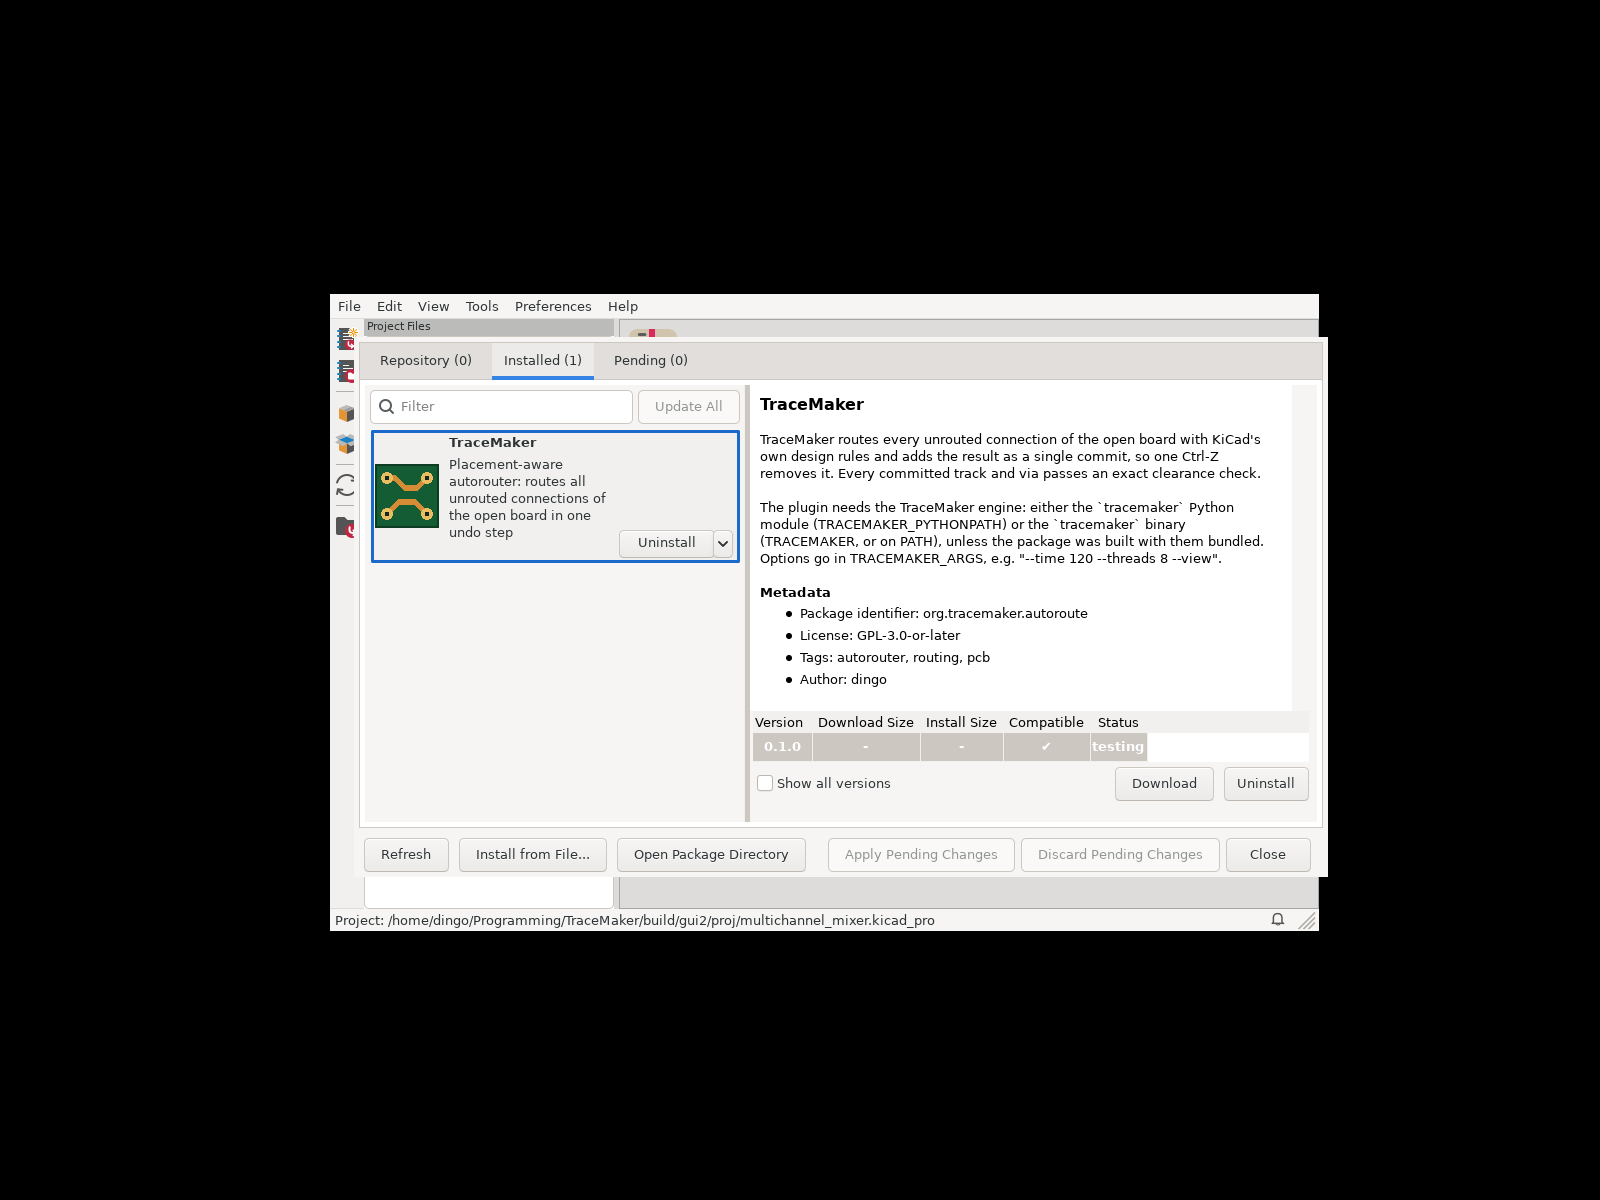
\includegraphics[width=0.62\linewidth,trim=330 265 270 290,clip]{pcm-installed.png}
\caption{KiCad's Plugin and Content Manager after ``Install from File'', captured from the virtual display.}
\label{fig:pcm}
\end{figure}

% ------------------------------------------------------------------------------------------------------------
\section{Experiments of the close-out}\label{sec:experiments}

Each row is one experiment: what was compared, on what, and the result. ``Fixed budget'' means \code{--work}, so
the numbers are repeatable to the connection.

{\small
\begin{longtable}{@{}p{0.17\linewidth}p{0.29\linewidth}p{0.33\linewidth}p{0.11\linewidth}@{}}
\caption{Experiments, 6 October 2026. Raw results are under \code{build/} and \code{bench/results/} in the files
named; the design documents give the full account (\code{docs/05-routing.md} \S16 to \S25,
\code{docs/04-placement.md} \S10).}\label{tab:experiments}\\
\toprule Experiment & Configuration & Result & Outcome \\ \midrule \endhead
Global congestion map & 18 hard boards, one variant, 100\,M expansions; map at three settings against none (\code{build/m6-cong2.txt}) & 13,285 routed without; 13,289 to 13,294 with; corridors 12,933 & off (D53) \\
Tile capacity model & boundary samples against the narrowest of eight cut lines & tiles at or above 75\,\% full on Aleste: 1.7\,\% $\to$ 4.3\,\% & kept \\
Group re-route of conflicting nets & up to five connections, every order; 8 nearly clean boards (all variants, 60\,M) and 24 boards (one variant) & identical routed count on every board & removed \\
Planning by copper distance & 24 boards, one variant, 60\,M (\code{build/m8-r4.txt}); then tiers & 11,905 $\to$ 11,986 routed (15 boards better, 4 worse); tiers A to D neutral, tier D side by side 16,618 $\to$ 16,622 & on (D54) \\
DRC profile on large zone boards & vme-wren (38,062 copper items, 128 zones), per-phase timing & broad-phase 14\,ms; exact tests against zone fills 650 of 730\,s & index built \\
Zone-fill edge index & vme-wren and jetson, indexed against linear path & 730\,s $\to$ 7\,s and 250\,s $\to$ 4\,s; reports byte-identical & on (D55) \\
Global router v2 & 18 hard boards, one variant, 100\,M (\code{build/m6-v2.txt}) & 13,305 without; 12,967 corridors; 12,735 confined; 13,324 map & off (D56) \\
Global routing time & per board, timing output & tile-graph routing 0.02 to 0.5\,s; set-up 0.4 to 1.3\,s & no GPU port \\
Cut-line proofs (R6) & 92 boards of tiers B to D (\code{build/cut-report-tiers.json}) & no over-full line; tightest line 9\,\% used at the median, 40\,\% at most & built, report only \\
Successive halving & 24 boards, 30\,M per thread, 2 and 4 threads (\code{build/m10-halving.txt}) & 12,385 and 12,451 against 12,402 and 12,508 for the first variants & off (D59) \\
Micro vias & two four-layer boards with the setting forced on, 20\,M & routing complete or unchanged; KiCad clean; none needed & built, off \\
Half the lattice pitch & 12 nearly clean boards, all variants, 30\,M against 120\,M at half pitch (\code{build/m12-pitch.txt}) & 4,140 $\to$ 4,153 routed; one more board complete; 9 better, 2 worse & one variant \\
Half-pitch variant on the tiers & tiers B and C, with and without, side by side (\code{ab-fine-*}, \code{ab-nofine-*}) & B 27 $\to$ 28 clean, 5,156 $\to$ 5,163; C 18 $\to$ 18, 9,506 $\to$ 9,514; no added errors & on (D63) \\
Pair twists & 18 boards, 59 pairs, one variant, 30\,M & one pair 0 $\to$ 86\,\% coupled, none worse; at least half coupled 35 $\to$ 36; median share 57 $\to$ 63\,\%; routed 2,210 $\to$ 2,212 & on (D64) \\
Why pairs fail & same boards, tagged first attempts & 63 of 120 attempts couple; 20 of 26 ``mirrored'' failures are one pair retried; 13 of 21 attempts joining routed copper couple & measured \\
Net classes from rules & StickHub, CM5 Minima, a unit test on a synthetic four-layer board & USB pair 0.760/0.150\,mm for 90\,$\Omega$; supply 1.367\,mm for 3\,A; exactly the two nets resolve to the class & built, opt-in (D58) \\
Part spacing on near misses & two S boards, courtyard clearance 0.6 and 1.0\,mm & fewer connections routed (pico-pi 216 $\to$ 211 and 191) & not adopted \\
\bottomrule
\end{longtable}
}

% ------------------------------------------------------------------------------------------------------------
\section{Faults found by testing}\label{sec:faults}

\begin{table}[H]
\centering\small
\begin{tabular}{@{}p{0.19\linewidth}p{0.35\linewidth}p{0.37\linewidth}@{}}
\toprule
Fault & How it was found & Fix and its test \\
\midrule
Copper routed across Margin-layer lines & Held-out board kitspace\_hack: KiCad reported 13 to 24 edge-clearance errors on new tracks, with the designer's placement too & Margin graphics are edges in the router and in TraceMaker's DRC; DRC parity tests; re-route adds no edge error \\
Hole-less pads connected on the far side & Held-out board Kefersender: the router reported 84 of 84, KiCad 2 unconnected & A pad without a hole has copper on its footprint's side only; KiCad then agrees (0 unconnected) \\
Failure reasons were stale & Reasons disagreed with what a single-board run showed & Reasons are saved with the best state; ripped connections name the net that ripped them \\
DRC took minutes on boards with large zones & Timing vme-wren for the broad-phase item & Edge index and rule cache, with the linear path kept as reference \\
Parts left stacked by from-scratch placement & Set S: shorts and courtyard overlaps in KiCad & \code{--scratch}; fallbacks never return to the input \\
Cut ``proof'' on MicroMaple was wrong & The proof contradicted routed results & Demand counts only pads wholly on either side with no pad across the line \\
Pair lost its coupling after a planning change & \code{diff\_pair} test failed & Runs with pair routing keep the old planning \\
A work-budget test depended on wall time & Sanitizer run on a loaded machine & Test passes \code{--time 3600} \\
\bottomrule
\end{tabular}
\caption{Faults found during the close-out. The first two were present in every earlier benchmark run.}
\end{table}

% ------------------------------------------------------------------------------------------------------------
\section{What is not tested or not measured}

\begin{itemize}
\item \textbf{M7's comparison with SA-PCB.} The baseline placer needs SWIG for its KiCad parser and its plain
  Makefile is stale; it was cloned (\code{build/tools/sa-pcb}) and not built.
\item \textbf{The viewer's frame rate.} No GPU-backed browser is available on the machine.
\item \textbf{The thread-sanitizer preset} was not run in the close-out, and the address-sanitizer preset was not
  rerun end to end after its slow tests were adjusted.
\item \textbf{The plugin's toolbar button in KiCad} after installation through the package manager.
\item \textbf{The last placer change} (mask openings as convex hulls) passed the test suite; set S was not rerun
  after it.
\item \textbf{Micro vias and per-layer widths} have no fixture that needs them; they are tested for correctness
  on boards with the setting forced, not for benefit.
\item \textbf{Three KiCad demo boards} still differ from KiCad's DRC in documented ways.
\item \textbf{Global-routing set-up on LeeChee} takes 135 seconds because obstacle queries are about fifty times
  slower on that board; the cause was not found. Only the opt-in global options are affected.
\end{itemize}

% ------------------------------------------------------------------------------------------------------------
\section{Roadmap in full}\label{sec:roadmapdetail}

Generated from \code{dev/progress.json}. A check mark is a closed task; its text says whether it was built or
closed without building, and with which result.

\subsection*{M0: Toolchain and skeleton}
\addcontentsline{toc}{subsection}{M0: Toolchain and skeleton}
\noindent\textbf{Deliverables.} CMake presets (\texttt{debug}, \texttt{release}, \texttt{asan}, \texttt{cpu-only}), CUDA build with a GCC host compiler that \texttt{nvcc 12.4} accepts, Catch2, clang-format/clang-tidy config (or GCC equivalents), \texttt{scripts/bootstrap.sh}, \texttt{kicad-cli} available (Docker image or native), fixture download script\par\smallskip
\noindent\textbf{Gate.} \texttt{ctest} runs a CPU and a CUDA hello-kernel test on both GPUs; \texttt{kicad-cli version} works from the harness\par\smallskip
\noindent\textbf{Tasks} (14 of 14 closed; status: done).
\begin{itemize}[leftmargin=1.6em,itemsep=1pt]
\item[\textcolor{fraqua}{$\checkmark$}] Ubuntu setup script (packages, Docker, KiCad 10 kicad-cli wrapper)
\item[\textcolor{fraqua}{$\checkmark$}] Git repository, .gitignore
\item[\textcolor{fraqua}{$\checkmark$}] CMake project + presets (debug, release, cpu-only, asan, tsan)
\item[\textcolor{fraqua}{$\checkmark$}] CUDA build: nvcc 12.4 with g++-13 host, sm\_60 + sm\_70; system GCC 15 for C++
\item[\textcolor{fraqua}{$\checkmark$}] Core library: units, deterministic Philox/SplitMix RNG
\item[\textcolor{fraqua}{$\checkmark$}] GPU service: device discovery by UUID, free-memory admission control
\item[\textcolor{fraqua}{$\checkmark$}] First kernel with CPU reference; bit-identical on V100 and P100
\item[\textcolor{fraqua}{$\checkmark$}] Catch2 tests wired into ctest with JUnit results
\item[\textcolor{fraqua}{$\checkmark$}] tracemaker CLI: version, gpu-info
\item[\textcolor{fraqua}{$\checkmark$}] Development progress website (0.0.0.0)
\item[\textcolor{fraqua}{$\checkmark$}] scripts/bootstrap.sh: configure, build and test all presets
\item[\textcolor{fraqua}{$\checkmark$}] Benchmark environment check (kicad-cli from the harness)
\item[\textcolor{fraqua}{$\checkmark$}] Fixture download script (Freerouting, DAC2020, KiCad demos, PCBench)
\item[\textcolor{fraqua}{$\checkmark$}] Gate: CPU + CUDA tests pass on both GPUs; kicad-cli works from harness
\end{itemize}
\subsection*{M1: KiCad I/O and board model}
\addcontentsline{toc}{subsection}{M1: KiCad I/O and board model}
\noindent\textbf{Deliverables.} s-expression lexer/parser/writer; \texttt{.kicad\_pcb}, \texttt{.kicad\_pro}, \texttt{.kicad\_dru}, \texttt{.kicad\_sch} (netlist), \texttt{.kicad\_mod}; board model with layers, stackup, footprints, pads, tracks, vias, zones, nets, net classes; DSN reader\par\smallskip
\noindent\textbf{Gate.} Byte-identical round-trip of every fixture board (parse $\to$ write); netlist equals \texttt{kicad-cli sch export netlist} on all fixture projects\par\smallskip
\noindent\textbf{Tasks} (11 of 11 closed; status: done).
\begin{itemize}[leftmargin=1.6em,itemsep=1pt]
\item[\textcolor{fraqua}{$\checkmark$}] Lossless s-expression parser/writer with span edits
\item[\textcolor{fraqua}{$\checkmark$}] Board reader: layers, nets (KiCad 9 and 10 syntax), footprints, pads, tracks, arcs, vias, zones, graphics
\item[\textcolor{fraqua}{$\checkmark$}] Reader verified against pcbnew ground truth on demo boards
\item[\textcolor{fraqua}{$\checkmark$}] Byte-identical round trip of fixture boards
\item[\textcolor{fraqua}{$\checkmark$}] Design rules: .kicad\_pro net classes, patterns, assignments, board minimums
\item[\textcolor{fraqua}{$\checkmark$}] Custom rules: .kicad\_dru parsed into rules and constraints
\item[\textcolor{fraqua}{$\checkmark$}] Board editor: add/remove tracks and vias, move/rotate footprints
\item[\textcolor{fraqua}{$\checkmark$}] Edited boards load in pcbnew with the expected geometry
\item[\textcolor{fraqua}{$\checkmark$}] Netlist import via kicad-cli (kicadsexpr) and cross-check against board pad nets
\item[\textcolor{fraqua}{$\checkmark$}] tracemaker inspect: board summary and JSON dump
\item[\textcolor{fraqua}{$\checkmark$}] Gate: round trip on all fixtures; reader matches KiCad
\end{itemize}
\subsection*{M2: Rules and DRC parity}
\addcontentsline{toc}{subsection}{M2: Rules and DRC parity}
\noindent\textbf{Deliverables.} Rule compiler (net classes, board constraints, custom rules subset), spatial indices, own DRC with KiCad violation names\par\smallskip
\noindent\textbf{Gate.} Same violation multiset as \texttt{kicad-cli pcb drc} on all unrouted and routed fixture boards (documented, tested exceptions only)\par\smallskip
\noindent\colorbox{boxfill}{\parbox{\dimexpr\linewidth-2\fboxsep}{\textbf{Gate result.} Result: 14 of 17 KiCad demo boards exact and 264 of 264 injected-defect variants (regression tests); three demo boards differ in documented ways. Since 2026-10-06 Margin-layer edges and one-sided SMD pads match KiCad too.}}\par\smallskip
\noindent\textbf{Tasks} (11 of 11 closed; status: done).
\begin{itemize}[leftmargin=1.6em,itemsep=1pt]
\item[\textcolor{fraqua}{$\checkmark$}] Exact integer geometry kernel (rounded-core shapes, int128 predicates, fine arc flattening)
\item[\textcolor{fraqua}{$\checkmark$}] Copper item model: pads (all shapes, drill offsets), tracks, arcs, vias, zone fills, copper graphics with nets
\item[\textcolor{fraqua}{$\checkmark$}] Rule engine: net classes, local overrides, diff pairs, board minimums, legacy rules, custom-rule conditions
\item[\textcolor{fraqua}{$\checkmark$}] Checks: clearance, shorts, crossings, widths, vias, annular, holes, edge, keepouts
\item[\textcolor{fraqua}{$\checkmark$}] Anchor/overlap connectivity, unconnected items, dangling tracks/vias
\item[\textcolor{fraqua}{$\checkmark$}] DRC parity harness vs kicad-cli + fuzzer
\item[\textcolor{fraqua}{$\checkmark$}] Parity: 11/16 demo boards exact (regression test)
\item[\textcolor{fraqua}{$\checkmark$}] Parity on broken-board classification (shorts/dangling): 264/264 injected-defect variants match kicad-cli violation by violation (was 41/264; regression test); demo boards 14/17 exact
\item[\textcolor{fraqua}{$\checkmark$}] Performance on very large boards: vme-wren 730 s -\textgreater{} 7 s, jetson 250 s -\textgreater{} 4 s (zone-fill edge index, area-rule cache; identical reports)
\item[\textcolor{fraqua}{$\checkmark$}] Copper text obstacle margin (estimated glyph boxes)
\item[\textcolor{fraqua}{$\checkmark$}] DRC parity 12 of 17 KiCad demo boards (jetson now exact; RoyalBlue54L down to a malformed duplicate pad)
\end{itemize}
\subsection*{M3: Event bus, server, viewer v1}
\addcontentsline{toc}{subsection}{M3: Event bus, server, viewer v1}
\noindent\textbf{Deliverables.} Event types, ring buffers, WebSocket server, FlatBuffers schema, replay log; WebGL2 viewer (WebGPU backend optional): layers, pan/zoom, pads/tracks/vias/zones, ratsnest, dark theme\par\smallskip
\noindent\textbf{Gate.} Viewer renders the largest fixture board at $\geq$ 60 fps; replay of a recorded log reproduces the final board\par\smallskip
\noindent\colorbox{boxfill}{\parbox{\dimexpr\linewidth-2\fboxsep}{\textbf{Gate result.} Result: replay reproduces the routed board (test record\_replay). The 60 fps figure was not measured: there is no GPU-backed browser on this machine.}}\par\smallskip
\noindent\textbf{Tasks} (9 of 9 closed; status: done).
\begin{itemize}[leftmargin=1.6em,itemsep=1pt]
\item[\textcolor{fraqua}{$\checkmark$}] Event types and Sink interface
\item[\textcolor{fraqua}{$\checkmark$}] WebSocket server (Boost.Beast), static files, snapshot + deltas, back-pressure
\item[\textcolor{fraqua}{$\checkmark$}] Viewer: WebGL2 instanced tracks/pads/vias/zones, layers, pan/zoom
\item[\textcolor{fraqua}{$\checkmark$}] Live effects: glow, frontiers, failures, HUD, log, tooltips
\item[\textcolor{fraqua}{$\checkmark$}] tracemaker-view with --demo
\item[\textcolor{fraqua}{$\checkmark$}] Router live streaming (route --view)
\item[\textcolor{fraqua}{$\checkmark$}] Replay log (zstd frames, --record FILE.zst) and heatmaps (expansions, history) live and in replay; test: recording/viewing leave the routed board byte-identical
\item[\textcolor{fraqua}{$\checkmark$}] Event recording (route --record) and replay (tracemaker-view --replay); test: replay reproduces the routed board exactly
\item[\textcolor{fraqua}{$\checkmark$}] FlatBuffers schema: closed, not built (protocol and replay log stay JSON, zstd-compressed logs 12-13x smaller; D45, D61)
\end{itemize}
\subsection*{M4: First router (lattice A*)}
\addcontentsline{toc}{subsection}{M4: First router (lattice A*)}
\noindent\textbf{Deliverables.} Rerun debug logging of searches (optional), transactions, scoring, union-find, bit-planes, A* + radix heap, insertion with exact validation, basic pull-tight; sequential routing in net order; \texttt{tracemaker route} CLI; bench harness v1 with KiCad-DRC judge and Freerouting runner\par\smallskip
\noindent\textbf{Gate.} Routes the simple fixture set with 0 added KiCad DRC errors; harness produces the comparison table\par\smallskip
\noindent\textbf{Tasks} (6 of 6 closed; status: done).
\begin{itemize}[leftmargin=1.6em,itemsep=1pt]
\item[\textcolor{fraqua}{$\checkmark$}] Router obstacle model with exact KiCad-rule legality
\item[\textcolor{fraqua}{$\checkmark$}] Octilinear lattice A* with vias, bends, admissible heuristic
\item[\textcolor{fraqua}{$\checkmark$}] Path simplification, exact verification, commit through the board editor
\item[\textcolor{fraqua}{$\checkmark$}] tracemaker route CLI
\item[\textcolor{fraqua}{$\checkmark$}] Benchmark harness judged by kicad-cli with Freerouting baselines
\item[\textcolor{fraqua}{$\checkmark$}] Gate: zero added KiCad DRC errors on the benchmark
\end{itemize}
\subsection*{M5: Failure memory T0--T2 + escalation R0--R3 + repair}
\addcontentsline{toc}{subsection}{M5: Failure memory T0--T2 + escalation R0--R3 + repair}
\noindent\textbf{Deliverables.} Failure records, Zobrist signatures, nogood store, history + targeted penalties, conflict graph, activity ordering, bandit; negotiated rip-up; repair windows; aggressor/victim repair\par\smallskip
\noindent\textbf{Gate.} Completion $\geq$ Freerouting on the Freerouting test set; ablation shows each learning mechanism helps or is removed\par\smallskip
\noindent\textbf{Tasks} (10 of 10 closed; status: done).
\begin{itemize}[leftmargin=1.6em,itemsep=1pt]
\item[\textcolor{fraqua}{$\checkmark$}] Negotiated rip-up and reroute (soft crossing of routed copper, victims requeued)
\item[\textcolor{fraqua}{$\checkmark$}] PathFinder history on contested cells
\item[\textcolor{fraqua}{$\checkmark$}] Learned blocked cells after exact-check failures
\item[\textcolor{fraqua}{$\checkmark$}] Best-state keeping
\item[\textcolor{fraqua}{$\checkmark$}] Failure records, nogoods, conflict graph, bandit (T0-T2 complete)
\item[\textcolor{fraqua}{$\checkmark$}] Gate: completion \textgreater{}= Freerouting on tier A (100\% clean, equal to Freerouting RC12, in every run since 2026-10-03)
\item[\textcolor{fraqua}{$\checkmark$}] Reverse probe for boxed-in targets; pad legs dropped when the lattice end is on the pad; learned blocks beside fine-pitch pads
\item[\textcolor{fraqua}{$\checkmark$}] Diversified extra restarts while budget remains
\item[\textcolor{fraqua}{$\checkmark$}] Post-routing clean-up: via-saving re-routes and path smoothing (bends -40\%, vias -25-33\%)
\item[\textcolor{fraqua}{$\checkmark$}] Connection planning by pad copper distance (--plan-gap, on, D54): 24 boards at a fixed budget 11,905 -\textgreater{} 11,986 routed; tiers A-D neutral; failure reasons now reported as at the best state
\end{itemize}
\subsection*{M6: Global routing + GPU}
\addcontentsline{toc}{subsection}{M6: Global routing + GPU}
\noindent\textbf{Deliverables.} Port/adapt GAMER sweep and GGR pattern kernels from Xplace \texttt{gpugr} (BSD-3); tile graph, Steiner decomposition, CPU NCR, corridors; GPU pattern routing, GPU sweep maze routing, GPU cost-to-go fields, GPU DRC broad-phase\par\smallskip
\noindent\textbf{Gate.} CPU and GPU results identical on every fixture; time-to-route reduced on dense boards with no quality loss\par\smallskip
\noindent\textbf{Tasks} (10 of 10 closed; status: done).
\begin{itemize}[leftmargin=1.6em,itemsep=1pt]
\item[\textcolor{fraqua}{$\checkmark$}] GPU cost-to-go fields (CUDA sweeps) with identical CPU reference
\item[\textcolor{fraqua}{$\checkmark$}] Fields used as the router's A* heuristic; deterministic with/without GPU
\item[\textcolor{fraqua}{$\checkmark$}] Coarse global routing + corridors (CPU, negotiated congestion): built, off by default (corridors cost completion in three measurements)
\item[\textcolor{fraqua}{$\checkmark$}] GPU pattern/maze global routing (GAMER/GGR port): closed, not built. The CPU global router routes the tile graph in 0.02-0.5 s per board and its plan does not help (D56)
\item[\textcolor{fraqua}{$\checkmark$}] GPU DRC broad-phase: closed, not built. Broad-phase is 14 ms; the DRC was fixed on the CPU with a zone-fill edge index: vme-wren 730 s -\textgreater{} 7 s, jetson 250 s -\textgreater{} 4 s, reports byte-identical (D55)
\item[\textcolor{fraqua}{$\checkmark$}] Adaptive GPU-field cut-off under GPU contention (wall-clock mode)
\item[\textcolor{fraqua}{$\checkmark$}] CPU global router v1 (tile graph, capacities, negotiated congestion, soft corridors): experimental, no gain yet
\item[\textcolor{fraqua}{$\checkmark$}] Global router v2: net-shared edges (Steiner demand), via capacity, layer-true corridors, integer costs, corridor-restricted windows: built; 18 hard boards 13,305 without, 12,967 corridors, 13,324 congestion map; off (D56)
\item[\textcolor{fraqua}{$\checkmark$}] Exact flood-fill reachability pre-check before likely-failing searches (10 hard boards +47 routed at fixed budget; tiers neutral)
\item[\textcolor{fraqua}{$\checkmark$}] Global congestion map + cut-based tile capacities (opt-in --global-congestion): 18 hard boards 13,285 -\textgreater{} 13,294 routed, within noise; kept off (D53). Boards are not congested at tile scale; v2 remainder deferred
\end{itemize}
\subsection*{M7: Placement A--D}
\addcontentsline{toc}{subsection}{M7: Placement A--D}
\noindent\textbf{Deliverables.} Constraint extraction, decoupling detection, quadratic B2B (PCG), electrostatic global placement (CPU then GPU batched), rotation/side assignment, LP legalisation; placement report with optimality levels and lower bound\par\smallskip
\noindent\textbf{Gate.} Placements are legal (zero courtyard overlaps, inside outline); HPWL $\leq$ SA-PCB baseline on the placement set\par\smallskip
\noindent\colorbox{boxfill}{\parbox{\dimexpr\linewidth-2\fboxsep}{\textbf{Gate result.} Result: legality met (held-out set, doc 04 \S10). The HPWL comparison with SA-PCB was NOT measured: the baseline does not build here (it needs SWIG, which is not installed, and its Makefile is stale; build/tools/sa-pcb).}}\par\smallskip
\noindent\textbf{Tasks} (12 of 12 closed; status: done).
\begin{itemize}[leftmargin=1.6em,itemsep=1pt]
\item[\textcolor{fraqua}{$\checkmark$}] Constraint extraction (fixed parts, outline, keepouts, courtyards, copper legality)
\item[\textcolor{fraqua}{$\checkmark$}] Decoupling capacitors tied to their IC supply pin (D25)
\item[\textcolor{fraqua}{$\checkmark$}] Other proximity groups: crystals, load caps, ESD near connectors, regulator caps (M13, --component-rules soft)
\item[\textcolor{fraqua}{$\checkmark$}] quadratic B2B (Eigen CG)
\item[\textcolor{fraqua}{$\checkmark$}] global spreading (SimPL instead of electrostatic; CPU)
\item[\textcolor{fraqua}{$\checkmark$}] Rotation assignment (coordinate descent)
\item[\textcolor{fraqua}{$\checkmark$}] Side assignment (flip to the back): opt-in --flip, annealer flip move + via estimate, KiCad-exact mirror (2,529 footprints = pcbnew); 23 boards HPWL -8\%, crossings -31\%, 0 new DRC (D48)
\item[\textcolor{fraqua}{$\checkmark$}] legalisation (greedy minimum displacement; LP not done)
\item[\textcolor{fraqua}{$\checkmark$}] parallel simulated annealing, deterministic across thread counts
\item[\textcolor{fraqua}{$\checkmark$}] placement report with optimality levels and LP lower bound (min-cost flow)
\item[\textcolor{fraqua}{$\checkmark$}] evaluation on 23 PCBench boards: HPWL -17..-26\% median, zero new DRC errors; routability not yet improved
\item[\textcolor{fraqua}{$\checkmark$}] --mode auto with route checks: 23 boards, HPWL -24.5\% total, never more unrouted (61 -\textgreater{} 59)
\end{itemize}
\subsection*{M8: Placement E--G + ECO}
\addcontentsline{toc}{subsection}{M8: Placement E--G + ECO}
\noindent\textbf{Deliverables.} GPU parallel-tempering SA, LNS, CP-SAT windows, routability loop; R4 exact window solve, R5 trial ordering, R6 cut proofs, ECO placement moves\par\smallskip
\noindent\textbf{Gate.} Schematic-to-board set: clean pass $\geq$ 90\%; \texttt{eco} mode closes boards that \texttt{none} mode cannot\par\smallskip
\noindent\colorbox{boxfill}{\parbox{\dimexpr\linewidth-2\fboxsep}{\textbf{Gate result.} Result 2026-10-06: NOT met. From-scratch clean pass 85 \% (34/40) on set S; 4 of the 6 failing boards cannot be clean in any placement. eco closed 0 of the 1 held-out board the human placement leaves unrouted (3 of 7 on the development set).}}\par\smallskip
\noindent\textbf{Tasks} (12 of 12 closed; status: done).
\begin{itemize}[leftmargin=1.6em,itemsep=1pt]
\item[\textcolor{fraqua}{$\checkmark$}] Parallel tempering (annealed replica exchange, CPU; deterministic for 1/3/16 threads): refine cost -4\% on 23 boards, full neutral
\item[\textcolor{fraqua}{$\checkmark$}] GPU parallel-tempering SA: closed, not built (annealing 1.9 s median, 56 s max on the held-out boards; CPU tempering neutral on routability; D57)
\item[\textcolor{fraqua}{$\checkmark$}] LNS (window rip-up, exact \textless{}=4 parts, greedy otherwise; never worsens)
\item[\textcolor{fraqua}{$\checkmark$}] Exact windows by branch and bound (CP-SAT not available; B\&B equals full enumeration)
\item[\textcolor{fraqua}{$\checkmark$}] CP-SAT windows: closed, not built (no OR-tools C++ library; exact windows by branch and bound equal full enumeration; D57)
\item[\textcolor{fraqua}{$\checkmark$}] RUDY routability term in the annealer (incremental, exact vs reference)
\item[\textcolor{fraqua}{$\checkmark$}] Routability loop (--mode routable): 23 boards unrouted 64 -\textgreater{} 35 (auto 60), 0 new DRC errors
\item[\textcolor{fraqua}{$\checkmark$}] ECO placement moves (--mode eco): closes 3 of 7 incomplete boards, unrouted 64 -\textgreater{} 48
\item[\textcolor{fraqua}{$\checkmark$}] Schematic-to-board set S (40 held-out boards, parts piled) built and the gate measured: 85 \% clean (34/40) with routable --scratch, human placement 95 \%; gate of 90 \% NOT met (doc 04 \S10)
\item[\textcolor{fraqua}{$\checkmark$}] R4 exact window solve: closed, not built as an exact model (no CP-SAT); the group re-route stand-in changed no board and was removed (doc 05 \S17, \S20)
\item[\textcolor{fraqua}{$\checkmark$}] R5 trial ordering: closed, not built (every order of small conflict groups was tried and changed no board, doc 05 \S17, \S20)
\item[\textcolor{fraqua}{$\checkmark$}] R6 cut proofs: built (route --cut-report); no over-full line on 92 tier B-D boards, tightest line 40 \% used
\end{itemize}
\subsection*{M9: Escape planning}
\addcontentsline{toc}{subsection}{M9: Escape planning}
\noindent\textbf{Deliverables.} Min-cost-flow escape, layer assignment, NC fallback, escape templates\par\smallskip
\noindent\textbf{Gate.} BGA boards in the academic set complete\par\smallskip
\noindent\colorbox{boxfill}{\parbox{\dimexpr\linewidth-2\fboxsep}{\textbf{Gate result.} Result: NOT met. 17 dense-package boards: 41 \% clean, 47 \% of the 15 feasible ones (Freerouting 2.5: 24 \%).}}\par\smallskip
\noindent\textbf{Tasks} (9 of 9 closed; status: done).
\begin{itemize}[leftmargin=1.6em,itemsep=1pt]
\item[\textcolor{fraqua}{$\checkmark$}] Escape corridors for dense-package pins (perimeter + dog-bone), opt-in --escape-plan
\item[\textcolor{fraqua}{$\checkmark$}] Escape feasibility analysis: tracemaker escape, dead pins with reasons and hints; benchmark dead\_pins / clean\_pass\_feasible
\item[\textcolor{fraqua}{$\checkmark$}] Via neck-down rung (smallest via the board minimums allow)
\item[\textcolor{fraqua}{$\checkmark$}] Dead pins: not retried after a negotiated neck-down check
\item[\textcolor{fraqua}{$\checkmark$}] Second-ring channel corridors (built, off: measured mixed)
\item[\textcolor{fraqua}{$\checkmark$}] Min-cost-flow channel assignment for deep arrays (built, opt-in --escape-flow: measured below the v1 corridors, D49)
\item[\textcolor{fraqua}{$\checkmark$}] Per-ring layer assignment (per pin, layer by layer, inside --escape-flow; same evidence, D49)
\item[\textcolor{fraqua}{$\checkmark$}] NC fallback for escapes: closed, not built (the flow planner it belongs to measured below the corridors and is off; ordinary negotiation already overrides corridors; D62)
\item[\textcolor{fraqua}{$\checkmark$}] Escape templates in the knowledge base: closed, not built (planning takes 0.1-2 s per board; a cache saves nothing; D62)
\end{itemize}
\subsection*{M10: Portfolio, determinism, knowledge base}
\addcontentsline{toc}{subsection}{M10: Portfolio, determinism, knowledge base}
\noindent\textbf{Deliverables.} Successive-halving portfolio, deterministic sync points, persistent KB (T3), warm starts\par\smallskip
\noindent\textbf{Gate.} Bit-identical output across thread counts and GPU on/off; clean pass up at fixed time budget\par\smallskip
\noindent\textbf{Tasks} (10 of 10 closed; status: done).
\begin{itemize}[leftmargin=1.6em,itemsep=1pt]
\item[\textcolor{fraqua}{$\checkmark$}] Parallel portfolio of 8 router variants, best kept
\item[\textcolor{fraqua}{$\checkmark$}] Deterministic work budget (byte-identical repeat runs)
\item[\textcolor{fraqua}{$\checkmark$}] Persistent knowledge base with variant bandit
\item[\textcolor{fraqua}{$\checkmark$}] Restarts that keep history
\item[\textcolor{fraqua}{$\checkmark$}] Successive-halving budget allocation (--halving, restart-based): 24 boards at 2 / 4 threads 12,385 / 12,451 routed against 12,402 / 12,508 for the first variants; kept off (D59)
\item[\textcolor{fraqua}{$\checkmark$}] Bit-identical across thread counts (portfolio selection; --variants, all 8 with --work, D47)
\item[\textcolor{fraqua}{$\checkmark$}] Portfolio early stop once a variant routes everything (wall-clock mode)
\item[\textcolor{fraqua}{$\checkmark$}] 2x lattice pitch for two variants on large boards
\item[\textcolor{fraqua}{$\checkmark$}] Quality benchmark vs Freerouting 2.5.0-RC12 and 1.9.0 on 60 held-out boards (bench/quality\_bench.py)
\item[\textcolor{fraqua}{$\checkmark$}] Held-out quality benchmark on tier C-like boards (heldC-1) and DAC2020
\end{itemize}
\subsection*{M11: KiCad integration}
\addcontentsline{toc}{subsection}{M11: KiCad integration}
\noindent\textbf{Deliverables.} IPC plugin (live board in pcbnew, one undoable commit), Python bindings, PCM package\par\smallskip
\noindent\textbf{Gate.} Round-trip in KiCad on the demo boards\par\smallskip
\noindent\textbf{Tasks} (8 of 8 closed; status: done).
\begin{itemize}[leftmargin=1.6em,itemsep=1pt]
\item[\textcolor{fraqua}{$\checkmark$}] IPC action plugin: save copy with project, route, add tracks/vias in one commit
\item[\textcolor{fraqua}{$\checkmark$}] Offline test against kicad-python 0.8
\item[\textcolor{fraqua}{$\checkmark$}] Round trip in a running KiCad GUI (headless: pcbnew in Docker under Xvfb, scripts/kicad\_gui\_roundtrip.py): tracks 140 -\textgreater{} 316 in the open board, one undo removes them, DRC of the saved board clean of new errors
\item[\textcolor{fraqua}{$\checkmark$}] Python bindings (pybind11): read\_board, route, emit\_items, drc; GIL released; CLI parity test
\item[\textcolor{fraqua}{$\checkmark$}] PCM package (scripts/make\_pcm\_package.py, validate\_pcm.py; passes kicad-python 0.8 validator)
\item[\textcolor{fraqua}{$\checkmark$}] Plugin uses the Python module when importable, binary otherwise
\item[\textcolor{fraqua}{$\checkmark$}] Install the PCM archive in a running KiCad GUI (Plugin and Content Manager, Install from File: listed as installed and compatible; venv creation and toolbar button not checked, no network in the container)
\item[\textcolor{fraqua}{$\checkmark$}] Plugin: footprint moves (TRACEMAKER\_PLACE), re-routing of existing unlocked copper (TRACEMAKER\_REROUTE, route --reroute), zone refill (TRACEMAKER\_REFILL); checked in the running GUI
\end{itemize}
\subsection*{M12: Advanced rules and arms}
\addcontentsline{toc}{subsection}{M12: Advanced rules and arms}
\noindent\textbf{Deliverables.} Differential pairs, length/skew tuning, blind/micro vias, gridless tile-plane arm, learned ordering/congestion models\par\smallskip
\noindent\textbf{Gate.} Each feature gated by its own benchmark subset; no regressions\par\smallskip
\noindent\textbf{Tasks} (12 of 12 closed; status: done).
\begin{itemize}[leftmargin=1.6em,itemsep=1pt]
\item[\textcolor{fraqua}{$\checkmark$}] Differential pairs: experimental --diff-pairs (rarely couples)
\item[\textcolor{fraqua}{$\checkmark$}] Differential pairs: proper coupled routing (v2, opt-in --diff-pairs, D50): coupled pair search with coupled vias, breakout legs, re-coupling, enclosed-pin check, --pair-skew-mm; 18 PCBench boards: 35 of 59 pairs \textgreater{}= 50 \% coupled at the rule gap, completion 2,201 -\textgreater{} 2,210; KiCad: no new error kinds (one more Margin-layer edge clearance on a board that has 27 with pairs off) (doc 05 \S15)
\item[\textcolor{fraqua}{$\checkmark$}] Differential pairs: twists (layer change with the sides swapped, on with pair routing: one of 59 pairs gains coupling, median share 57 -\textgreater{} 63 \%), per-pair skew limits from component rules; pairs ending on routed copper measured to matter little (13 of 21 such attempts couple) and not built (D64)
\item[\textcolor{fraqua}{$\checkmark$}] Length and skew tuning (KiCad length constraints)
\item[\textcolor{fraqua}{$\checkmark$}] Blind/buried vias: experimental --blind-vias
\item[\textcolor{fraqua}{$\checkmark$}] Micro vias (--micro-vias, off): outer layer to the next at the class's microvia size where a through via is blocked; no fixture allows them on more than two layers; KiCad-clean on two boards with the setting forced on
\item[\textcolor{fraqua}{$\checkmark$}] Gridless tile-plane arm: closed, not built; a half-pitch portfolio variant for small boards takes its place (12 boards 4,140 -\textgreater{} 4,153 routed at half pitch; tier B 27 -\textgreater{} 28 clean; D63)
\item[\textcolor{fraqua}{$\checkmark$}] Learned ordering/congestion models: closed, not built (ordering changes measured no effect, tile congestion absent, variant bandit already in the knowledge base; D64)
\item[\textcolor{fraqua}{$\checkmark$}] Length tuning: custom length rules read; trombone meanders until in range; KiCad-judged test
\item[\textcolor{fraqua}{$\checkmark$}] Differential pairs: coupled pair routing v1 (experimental, --diff-pairs; rarely succeeds without coupled escapes)
\item[\textcolor{fraqua}{$\checkmark$}] Skew tuning for differential pairs (custom skew rules, inDiffPair condition)
\item[\textcolor{fraqua}{$\checkmark$}] Blind/buried vias where through vias are blocked (--blind-vias; correct on the 3 boards that allow them, no measurable gain)
\end{itemize}
\subsection*{M13: Component-aware layout rules}
\addcontentsline{toc}{subsection}{M13: Component-aware layout rules}
\noindent\textbf{Deliverables.} Category detection (USB, Ethernet, crystals, regulators, RF, ...), role binding, rule catalogue compiled into net classes, a sidecar .kicad\_dru, keep-outs and placer pseudo-nets; stackup impedance; report (doc 15)\par\smallskip
\noindent\textbf{Gate.} Detection precision/recall on a labelled PCBench subset; every applied rule met or reported; no regression on the quick tier\par\smallskip
\noindent\textbf{Tasks} (17 of 17 closed; status: done).
\begin{itemize}[leftmargin=1.6em,itemsep=1pt]
\item[\textcolor{fraqua}{$\checkmark$}] Verify the 41 unchecked catalogue numbers against their sources (2026-10-05: 9 confirmed, 9 corrected, 11 TraceMaker defaults now D, 12 unverifiable stay R; doc 15 \S8.10, D46)
\item[\textcolor{fraqua}{$\checkmark$}] Category detection + role binding with confidence
\item[\textcolor{fraqua}{$\checkmark$}] Rule compiler: sidecar .kicad\_dru, keep-out areas, placer pseudo-nets
\item[\textcolor{fraqua}{$\checkmark$}] Rule compiler: net classes from rules, used by the router with --component-rules on (tmk\_\textless{}RULE\textgreater{}\_\textless{}ref\textgreater{}, Default-class nets only, D58; doc 15 \S15)
\item[\textcolor{fraqua}{$\checkmark$}] Stackup parsing + impedance (IPC-2141A / Wadell) - widths/gaps reported per layer (P4, report only)
\item[\textcolor{fraqua}{$\checkmark$}] Detection and rule report
\item[\textcolor{fraqua}{$\checkmark$}] Labelled PCBench subset and benchmark
\item[\textcolor{fraqua}{$\checkmark$}] Placer pseudo-nets for proximity rules (crystal, ESD, regulator caps, generalised decoupling): --component-rules
\item[\textcolor{fraqua}{$\checkmark$}] Generated keep-outs (crystal, inductor) for router/DRC + sidecar .kicad\_dru
\item[\textcolor{fraqua}{$\checkmark$}] Per-net coupled routing for USB 2.0 pairs (RouterOptions::pair\_nets)
\item[\textcolor{fraqua}{$\checkmark$}] Net classes from rules: impedance width/gap from the stackup, IPC-2221 width for current, minimum widths (one width per net: front-layer solution; per-layer widths not built)
\item[\textcolor{fraqua}{$\checkmark$}] IPC-2221 width for current reported for rules with a current (USBC-09)
\item[\textcolor{fraqua}{$\checkmark$}] User override file (--rules-override, JSON): disable / assert / deny / set, validated, reported (doc 15 \S6.3)
\item[\textcolor{fraqua}{$\checkmark$}] Ethernet magnetics void (ETH-05) as a generated keep-out (--component-rules on)
\item[\textcolor{fraqua}{$\checkmark$}] Connector edge attraction in the placer (opt-in --edge-attraction, objective only)
\item[\textcolor{fraqua}{$\checkmark$}] Two-stage soft placement (decaps and their ICs locked first, D43)
\item[\textcolor{fraqua}{$\checkmark$}] Turn component rules on by default for placement (soft; placed tiers B+C off vs soft: clean pass unchanged, crystals closer, decaps equal; D52). Routing stays off
\end{itemize}


\appendix
% ------------------------------------------------------------------------------------------------------------
\section{Every test}\label{sec:alltests}

Release build, the full run that produced Table~\ref{tab:testsummary}. Unit tests are grouped by source file with
their Catch2 tags; integration tests carry their CTest labels and a description.

{\small
\subsection*{src/\allowbreak{}crules/\allowbreak{}test\_\allowbreak{}crules.cpp (19 tests, 0.3 s)}
\begin{longtable}{@{}p{0.57\linewidth}p{0.19\linewidth}rl@{}}
\toprule Test & Tags / labels & Time (s) & Result \\ \midrule \endhead
catalogue: embedded JSON loads with every category and rule & {\footnotesize [crules]} & 0.01 & passed \\
catalogue: schema errors are reported, not ignored & {\footnotesize [crules]} & 0.00 & passed \\
names: references, supplies, voltages, capacitances & {\footnotesize [crules]} & 0.00 & passed \\
detection and role binding on a synthetic board with pin names & {\footnotesize [crules]} & 0.01 & passed \\
detection is deterministic and independent of footprint order & {\footnotesize [crules]} & 0.02 & passed \\
boards without pin names: binding by nets and pad numbers, capped confidence & {\footnotesize [crules]} & 0.01 & passed \\
D25 ties are reproduced and the generalised decoupling is a superset & {\footnotesize [crules]} & 0.00 & passed \\
evaluation: proximity measured, statuses follow the mode & {\footnotesize [crules]} & 0.01 & passed \\
placement affinities: each part pulled by one rule, locked parts never & {\footnotesize [crules]} & 0.02 & passed \\
keep-outs: crystal area on the free layer, tracks only, named; sidecar rule & {\footnotesize [crules]} & 0.01 & passed \\
USB 2.0 pairs for coupled routing (USB2-02) & {\footnotesize [crules]} & 0.01 & passed \\
PCBench fixture: detection report is stable and finds the crystal & {\footnotesize [crules][fixture]} & 0.05 & passed \\
overrides: every form parses, in file order & {\footnotesize [crules][overrides]} & 0.01 & passed \\
overrides: typos and contradictions are errors with a clear message & {\footnotesize [crules][overrides]} & 0.01 & passed \\
overrides: disable a rule, a rule on one part, a category & {\footnotesize [crules][overrides]} & 0.02 & passed \\
overrides: deny and assert change which instances exist & {\footnotesize [crules][overrides]} & 0.01 & passed \\
overrides: set changes parameters; @REF wins over global, later wins among equals & {\footnotesize [crules][overrides]} & 0.02 & passed \\
ethernet: discrete magnetics bound and voided on the adjacent layer (ETH-05) & {\footnotesize [crules][ethernet]} & 0.01 & passed \\
ethernet: four layers, MagJack, through-hole magnetics & {\footnotesize [crules][ethernet]} & 0.01 & passed \\
\bottomrule\end{longtable}
\subsection*{src/\allowbreak{}crules/\allowbreak{}test\_\allowbreak{}impedance.cpp (16 tests, 0.1 s)}
\begin{longtable}{@{}p{0.57\linewidth}p{0.19\linewidth}rl@{}}
\toprule Test & Tags / labels & Time (s) & Result \\ \midrule \endhead
elliptic integral ratio K(k)/K(k') & {\footnotesize [impedance]} & 0.00 & passed \\
microstrip: Hammerstad \& Jensen against textbook, KiCad and IPC-2141A & {\footnotesize [impedance]} & 0.00 & passed \\
microstrip: 50 ohm on 1.6 mm FR-4 is about 3 mm wide (doc 15 \S5.3) & {\footnotesize [impedance]} & 0.00 & passed \\
stripline: Cohn/Wheeler against textbook and KiCad & {\footnotesize [impedance]} & 0.00 & passed \\
coupled microstrip: Kirschning \& Jansen against KiCad & {\footnotesize [impedance]} & 0.00 & passed \\
coupled stripline: Cohn 1955 exact and against KiCad & {\footnotesize [impedance]} & 0.00 & passed \\
grounded coplanar waveguide: exact and against KiCad & {\footnotesize [impedance]} & 0.00 & passed \\
impedance is monotone where the solver relies on it & {\footnotesize [impedance]} & 0.00 & passed \\
solving: integer-nm bisection round trips and is deterministic & {\footnotesize [impedance]} & 0.00 & passed \\
propagation delay & {\footnotesize [impedance]} & 0.00 & passed \\
IPC-2221 width for current & {\footnotesize [impedance][current]} & 0.00 & passed \\
stackup geometry: microstrip outside, stripline inside, reference zones & {\footnotesize [impedance][stackup]} & 0.00 & passed \\
impedance rules: widths per layer with a stackup, never without one & {\footnotesize [impedance][stackup]} & 0.01 & passed \\
width for current from a rule's current, with the stackup's copper & {\footnotesize [impedance][current]} & 0.01 & passed \\
KiCad demo stackups parse and give sane geometry & {\footnotesize [impedance][stackup][fixture]} & 0.04 & passed \\
net classes from rules: computed widths become classes for Default-class nets only & {\footnotesize [impedance][stackup][netclass]} & 0.01 & passed \\
\bottomrule\end{longtable}
\subsection*{src/\allowbreak{}place/\allowbreak{}test\_\allowbreak{}place.cpp (28 tests, 30.4 s)}
\begin{longtable}{@{}p{0.57\linewidth}p{0.19\linewidth}rl@{}}
\toprule Test & Tags / labels & Time (s) & Result \\ \midrule \endhead
rot90 matches KiCad rotation & {\footnotesize [place]} & 0.01 & passed \\
convex hull & {\footnotesize [place]} & 0.00 & passed \\
power-like net names & {\footnotesize [place]} & 0.00 & passed \\
ground-like net names & {\footnotesize [place]} & 0.00 & passed \\
translated closer() agrees with geom::closer\_than & {\footnotesize [place]} & 0.01 & passed \\
min-cost flow on a small graph & {\footnotesize [place]} & 0.00 & passed \\
HPWL lower bound is exact on a chain and bounds random placements & {\footnotesize [place]} & 0.01 & passed \\
raster fast path is conservative (raster free implies exactly legal) & {\footnotesize [place]} & 0.12 & passed \\
legalisation removes every overlap & {\footnotesize [place]} & 0.64 & passed \\
recording a placement never changes it & {\footnotesize [place]} & 3.07 & passed \\
full pipeline: legal, deterministic, incremental cost exact & {\footnotesize [place]} & 6.95 & passed \\
rotation descent is monotone & {\footnotesize [place]} & 0.00 & passed \\
extraction from a KiCad board & {\footnotesize [place][fixture]} & 0.02 & passed \\
decoupling capacitors are tied to an IC supply pin, objective only & {\footnotesize [place][fixture]} & 0.01 & passed \\
component-rule proximity pseudo-nets are objective only and skip D25-tied parts & {\footnotesize [place][fixture][crules]} & 0.03 & passed \\
edge pulls: one-pin anchored nets, exact incremental cost, objective only & {\footnotesize [place][crules]} & 2.94 & passed \\
edge pulls from component rules: movable connectors only, objective only & {\footnotesize [place][fixture][crules]} & 0.03 & passed \\
RUDY map: capacity inside the outline, scaling, incremental demand equals the reference & {\footnotesize [place][m8]} & 1.09 & passed \\
parallel tempering: legal, exact cost, identical for any thread count & {\footnotesize [place][m8]} & 4.59 & passed \\
LNS never worsens the cost and keeps the placement legal & {\footnotesize [place][m8]} & 1.99 & passed \\
exact window: branch and bound equals full enumeration and never worsens & {\footnotesize [place][m8]} & 0.83 & passed \\
ECO: only improving moves, locked parts never move, legal & {\footnotesize [place][m8]} & 0.65 & passed \\
P5: byte-identical board for 1, 3 and 16 threads (tempering + LNS + RUDY, refine) & {\footnotesize [place][m8][fixture]} & 4.11 & passed \\
routability loop: never worse than its best seed, locked parts fixed & {\footnotesize [place][m8]} & 1.54 & passed \\
flip: the placer's mirrored geometry is what the KiCad writer produces & {\footnotesize [place][fixture][flip]} & 0.02 & passed \\
flip: legal, exact incremental cost with the via term, deterministic, only allowed parts flip & {\footnotesize [place][fixture][flip]} & 1.09 & passed \\
flip: with no part allowed to flip, --flip changes nothing & {\footnotesize [place][flip]} & 0.62 & passed \\
flip: swap states exchange absolute poses on either side & {\footnotesize [place][flip]} & 0.00 & passed \\
\bottomrule\end{longtable}
\subsection*{src/\allowbreak{}server/\allowbreak{}test\_\allowbreak{}replay.cpp (5 tests, 5.2 s)}
\begin{longtable}{@{}p{0.57\linewidth}p{0.19\linewidth}rl@{}}
\toprule Test & Tags / labels & Time (s) & Result \\ \midrule \endhead
replay log round-trips plain and zstd & {\footnotesize [replay]} & 0.09 & passed \\
replay log keeps empty lines, long lines and end\_frame boundaries & {\footnotesize [replay]} & 0.02 & passed \\
a truncated compressed log yields its complete lines, a corrupt one throws & {\footnotesize [replay]} & 0.08 & passed \\
heat grid sizing, scaling and message & {\footnotesize [heatmap]} & 0.01 & passed \\
router heatmaps: emitted with a sink, routing unchanged by it & {\footnotesize [heatmap][route]} & 5.00 & passed \\
\bottomrule\end{longtable}
\subsection*{src/\allowbreak{}server/\allowbreak{}test\_\allowbreak{}server.cpp (4 tests, 0.4 s)}
\begin{longtable}{@{}p{0.57\linewidth}p{0.19\linewidth}rl@{}}
\toprule Test & Tags / labels & Time (s) & Result \\ \midrule \endhead
message builders put type first and classify & {\footnotesize [server]} & 0.00 & passed \\
board snapshot of pic\_programmer has the board's objects & {\footnotesize [server]} & 0.03 & passed \\
viewer server serves files, streams snapshot then deltas, shuts down & {\footnotesize [server]} & 0.01 & passed \\
slow clients lose transient messages but not state & {\footnotesize [server]} & 0.33 & passed \\
\bottomrule\end{longtable}
\subsection*{tests/\allowbreak{}test\_\allowbreak{}diff\_\allowbreak{}pair.cpp (5 tests, 0.0 s)}
\begin{longtable}{@{}p{0.57\linewidth}p{0.19\linewidth}rl@{}}
\toprule Test & Tags / labels & Time (s) & Result \\ \midrule \endhead
pair rule: tightest legal coupling without diff-pair settings & {\footnotesize [diffpair]} & 0.00 & passed \\
pair rule: net-class diff-pair width and gap, relaxed clearance only for KiCad pairs & {\footnotesize [diffpair]} & 0.00 & passed \\
pair rule: a custom diff\_pair\_gap rule wins, diff\_pair\_uncoupled limits the legs & {\footnotesize [diffpair]} & 0.01 & passed \\
pair geometry: offsets are symmetric and miters keep the offset distance & {\footnotesize [diffpair]} & 0.00 & passed \\
pair measurement: coupled share, gap and skew & {\footnotesize [diffpair]} & 0.00 & passed \\
\bottomrule\end{longtable}
\subsection*{tests/\allowbreak{}test\_\allowbreak{}escape.cpp (5 tests, 3.1 s)}
\begin{longtable}{@{}p{0.57\linewidth}p{0.19\linewidth}rl@{}}
\toprule Test & Tags / labels & Time (s) & Result \\ \midrule \endhead
escape plan: perimeter pins fan out, inner balls get one dog-bone site each & {\footnotesize [escape]} & 0.00 & passed \\
escape analysis: sbc's DRAM balls are blocked only by the solder-mask rule & {\footnotesize [escape][fixture]} & 3.12 & passed \\
escape flow: a 6 x 6 array escapes on its pad layer within every channel's capacity & {\footnotesize [escape]} & 0.01 & passed \\
escape flow: without channels between balls, inner rings take dog-bone vias and leave on the next layer & {\footnotesize [escape]} & 0.01 & passed \\
escape flow: shallow packages are planned exactly as version 1 & {\footnotesize [escape]} & 0.00 & passed \\
\bottomrule\end{longtable}
\subsection*{tests/\allowbreak{}test\_\allowbreak{}geom.cpp (7 tests, 0.6 s)}
\begin{longtable}{@{}p{0.57\linewidth}p{0.19\linewidth}rl@{}}
\toprule Test & Tags / labels & Time (s) & Result \\ \midrule \endhead
rotation follows KiCad's convention and is exact for right angles & {\footnotesize [geom]} & 0.00 & passed \\
segment intersection handles crossing, touching and collinear cases & {\footnotesize [geom]} & 0.00 & passed \\
exact closer-than agrees with floating-point distance away from the boundary & {\footnotesize [geom]} & 0.01 & passed \\
shape gaps: round pads, tracks and polygons & {\footnotesize [geom]} & 0.00 & passed \\
arcs flatten within the error bound & {\footnotesize [geom]} & 0.00 & passed \\
polygon edge index answers disk tests exactly like closer\_than & {\footnotesize [geom]} & 0.08 & passed \\
polygon edge index answers shape tests and gaps exactly like the linear reference & {\footnotesize [geom]} & 0.52 & passed \\
\bottomrule\end{longtable}
\subsection*{tests/\allowbreak{}test\_\allowbreak{}gpu.cpp (4 tests, 2.0 s)}
\begin{longtable}{@{}p{0.57\linewidth}p{0.19\linewidth}rl@{}}
\toprule Test & Tags / labels & Time (s) & Result \\ \midrule \endhead
CPU reference fill is deterministic & {\footnotesize [gpu][cpu-reference]} & 0.00 & passed \\
GPU Philox fill is bit-identical to the CPU reference on every device & {\footnotesize [gpu][cuda]} & 0.68 & passed \\
cost-to-go field: CPU reference is the exact shortest-path distance on a small case & {\footnotesize [gpu][field]} & 0.01 & passed \\
cost-to-go field: GPU equals CPU on random grids & {\footnotesize [gpu][field][cuda]} & 1.30 & passed \\
\bottomrule\end{longtable}
\subsection*{tests/\allowbreak{}test\_\allowbreak{}kicad\_\allowbreak{}io.cpp (8 tests, 0.4 s)}
\begin{longtable}{@{}p{0.57\linewidth}p{0.19\linewidth}rl@{}}
\toprule Test & Tags / labels & Time (s) & Result \\ \midrule \endhead
demo boards round-trip byte for byte & {\footnotesize [kicad][io]} & 0.14 & passed \\
board reader matches KiCad's own model & {\footnotesize [kicad][io]} & 0.16 & passed \\
reading an edited document gives the edited board & {\footnotesize [kicad][io]} & 0.03 & passed \\
stackup: layers, sublayers, permittivity and copper mapping are read; text is untouched & {\footnotesize [kicad][io][stackup]} & 0.00 & passed \\
stackup: boards without one say so; missing permittivity makes the gap incomplete & {\footnotesize [kicad][io][stackup]} & 0.01 & passed \\
stackup: KiCad demo with dielectric sublayers round-trips & {\footnotesize [kicad][io][stackup]} & 0.08 & passed \\
flipping a footprint: KiCad's mirror, layers swapped, the rest byte for byte & {\footnotesize [kicad][io][flip]} & 0.00 & passed \\
flipping a KiCad 5 module: user copper names, signed arc sweeps & {\footnotesize [kicad][io][flip]} & 0.00 & passed \\
\bottomrule\end{longtable}
\subsection*{tests/\allowbreak{}test\_\allowbreak{}netlist.cpp (1 tests, 0.0 s)}
\begin{longtable}{@{}p{0.57\linewidth}p{0.19\linewidth}rl@{}}
\toprule Test & Tags / labels & Time (s) & Result \\ \midrule \endhead
schematic netlist agrees with the board's pad nets & {\footnotesize [netlist][kicad]} & 0.01 & passed \\
\bottomrule\end{longtable}
\subsection*{tests/\allowbreak{}test\_\allowbreak{}rng.cpp (2 tests, 0.0 s)}
\begin{longtable}{@{}p{0.57\linewidth}p{0.19\linewidth}rl@{}}
\toprule Test & Tags / labels & Time (s) & Result \\ \midrule \endhead
Philox4x32-10 matches the Random123 known-answer vectors & {\footnotesize [core][rng]} & 0.00 & passed \\
RNG streams are pure functions of (seed, stage, item, n) & {\footnotesize [core][rng]} & 0.00 & passed \\
\bottomrule\end{longtable}
\subsection*{tests/\allowbreak{}test\_\allowbreak{}rules.cpp (4 tests, 0.0 s)}
\begin{longtable}{@{}p{0.57\linewidth}p{0.19\linewidth}rl@{}}
\toprule Test & Tags / labels & Time (s) & Result \\ \midrule \endhead
lengths with units convert to nanometres & {\footnotesize [rules]} & 0.00 & passed \\
net-class wildcard patterns & {\footnotesize [rules]} & 0.00 & passed \\
project net classes, patterns and minimums are read & {\footnotesize [rules]} & 0.01 & passed \\
classes inherit null values from Default; explicit assignments and custom rules are read & {\footnotesize [rules]} & 0.01 & passed \\
\bottomrule\end{longtable}
\subsection*{tests/\allowbreak{}test\_\allowbreak{}sexpr.cpp (7 tests, 0.0 s)}
\begin{longtable}{@{}p{0.57\linewidth}p{0.19\linewidth}rl@{}}
\toprule Test & Tags / labels & Time (s) & Result \\ \midrule \endhead
millimetre strings convert to nanometres exactly & {\footnotesize [sexpr]} & 0.01 & passed \\
documents parse into a navigable tree & {\footnotesize [sexpr]} & 0.01 & passed \\
unmodified documents write back byte for byte & {\footnotesize [sexpr]} & 0.00 & passed \\
malformed documents raise ParseError with a line number & {\footnotesize [sexpr]} & 0.01 & passed \\
edits remove, replace and append with KiCad indentation & {\footnotesize [sexpr]} & 0.00 & passed \\
append to an inline list moves the closing paren to its own line & {\footnotesize [sexpr]} & 0.00 & passed \\
replacing the same node twice keeps the last replacement & {\footnotesize [sexpr]} & 0.00 & passed \\
\bottomrule\end{longtable}
\subsection*{tests/\allowbreak{}test\_\allowbreak{}units.cpp (1 tests, 0.0 s)}
\begin{longtable}{@{}p{0.57\linewidth}p{0.19\linewidth}rl@{}}
\toprule Test & Tags / labels & Time (s) & Result \\ \midrule \endhead
millimetre \textless{}-\textgreater{} nanometre conversion is exact for KiCad values & {\footnotesize [core][units]} & 0.00 & passed \\
\bottomrule\end{longtable}
\subsection*{integration (tests/\allowbreak{}CMakeLists.txt) (16 tests, 261.6 s)}
\begin{longtable}{@{}p{0.57\linewidth}p{0.19\linewidth}rl@{}}
\toprule Test & Tags / labels & Time (s) & Result \\ \midrule \endhead
kicad\_\allowbreak{}edit\_\allowbreak{}roundtrip\newline{\footnotesize\color{ink2} Boards edited by TraceMaker (tracks and vias added, footprints moved and rotated) are read back by pcbnew in Docker; geometry must equal TraceMaker's own reading. Time limit 600 s.} & {\footnotesize kicad;integration} & 4.06 & passed \\
kicad\_\allowbreak{}drc\_\allowbreak{}parity\newline{\footnotesize\color{ink2} TraceMaker's DRC against \texttt{kicad-cli pcb drc} on 14 KiCad demo boards: the same violations, type by type (15 routing-relevant types). Time limit 1200 s.} & {\footnotesize kicad;integration} & 9.56 & passed \\
kicad\_\allowbreak{}drc\_\allowbreak{}broken\_\allowbreak{}parity\newline{\footnotesize\color{ink2} 264 boards with injected defects (11 demo boards, 12 defect kinds, 2 seeds): TraceMaker's DRC must match KiCad violation by violation. Time limit 1800 s.} & {\footnotesize kicad;integration} & 35.91 & passed \\
drc\_\allowbreak{}zone\_\allowbreak{}index\newline{\footnotesize\color{ink2} DRC reports through the zone-fill edge index are byte-identical to the linear reference path (\texttt{drc -{}-linear-zones}) on four zone boards. Time limit 1800 s.} & {\footnotesize integration} & 21.69 & passed \\
global\_\allowbreak{}route\newline{\footnotesize\color{ink2} \texttt{route -{}-global} and \texttt{-{}-global-congestion} are repeatable byte for byte at a fixed work budget and stay within 5 connections of routing without them. Time limit 1800 s.} & {\footnotesize integration;route} & 15.98 & passed \\
record\_\allowbreak{}replay\newline{\footnotesize\color{ink2} A board routed plainly, with \texttt{-{}-record} and with \texttt{-{}-view} is byte-identical; replaying the recorded log reproduces the routed board. Time limit 600 s.} & {\footnotesize integration} & 12.11 & passed \\
python\_\allowbreak{}bindings\newline{\footnotesize\color{ink2} The Python module reads, routes, checks and emits items; \texttt{route} gives the same bytes as the CLI. Time limit 600 s.} & {\footnotesize python;integration} & 12.20 & passed \\
pcm\_\allowbreak{}package\newline{\footnotesize\color{ink2} Builds the KiCad PCM archive and validates its layout and metadata (also with kicad-python's validator). Time limit 120 s.} & {\footnotesize kicad} & 0.18 & passed \\
length\_\allowbreak{}tuning\newline{\footnotesize\color{ink2} A net with a custom \texttt{length} rule is meandered into range; KiCad's DRC judges the result. Time limit 600 s.} & {\footnotesize kicad;integration} & 3.40 & passed \\
crules\_\allowbreak{}catalogue\_\allowbreak{}sync\newline{\footnotesize\color{ink2} The committed rule catalogue JSON equals \texttt{docs/component\_rules.yaml} and the rule ids used in doc 15. Time limit 60 s.} & {\footnotesize crules} & 0.36 & passed \\
crules\_\allowbreak{}route\newline{\footnotesize\color{ink2} Routing with \texttt{-{}-component-rules on}: no new track enters a generated keep-out, the keep-outs are not written into the board, the sidecar \texttt{.kicad\_dru} is written. Time limit 600 s.} & {\footnotesize crules;integration} & 6.64 & passed \\
crules\_\allowbreak{}dru\_\allowbreak{}parses\newline{\footnotesize\color{ink2} KiCad itself parses the generated sidecar \texttt{.kicad\_dru} without errors. Time limit 900 s.} & {\footnotesize kicad;integration} & 5.02 & passed \\
crules\_\allowbreak{}two\_\allowbreak{}stage\newline{\footnotesize\color{ink2} Two-stage placement with component rules: the result is legal, and parts locked after stage 1 are where the decoupling-only placement put them. Time limit 3600 s.} & {\footnotesize integration} & 64.96 & passed \\
reach\_\allowbreak{}verify\newline{\footnotesize\color{ink2} Every ''unreachable'' verdict of the flood-fill pre-check is re-checked by the full A*: zero mismatches. Time limit 600 s.} & {\footnotesize route;integration} & 12.64 & passed \\
thread\_\allowbreak{}determinism\newline{\footnotesize\color{ink2} The same \texttt{-{}-work} portfolio at 1, 3 and 8 threads (and with fewer variants) writes identical bytes. Time limit 3600 s.} & {\footnotesize route;integration} & 29.77 & passed \\
diff\_\allowbreak{}pair\newline{\footnotesize\color{ink2} A USB hub's five differential pairs are routed coupled at the rule's gap, twice with identical bytes, and KiCad's DRC is clean. Time limit 3600 s.} & {\footnotesize route;kicad;integration} & 27.13 & passed \\
\bottomrule\end{longtable}

}

% ------------------------------------------------------------------------------------------------------------
\section{Final tier runs, board by board}\label{sec:perboard}

Runs \code{final11-tierA} to \code{final11-tierD}: eight variants, 120 seconds, KiCad's DRC as judge. The last
column is Freerouting 2.5.0-RC12's published result for the same board.

{\small
\subsection*{Tier A: 40 of 40 clean, 2637 of 2637 connections}
\begin{longtable}{@{}p{0.36\linewidth}rrrrcp{0.22\linewidth}@{}}
\toprule Board & Conn. & Routed & Vias & Time (s) & Clean & Freerouting 2.5 \\ \midrule \endhead
655\_\allowbreak{}testboard & 57 & 57 & 33 & 29 & \textcolor{fraqua}{yes} & {\footnotesize clean} \\
atmel-\allowbreak{}programmer\_\allowbreak{}atmel\_\allowbreak{}programmer & 39 & 39 & 5 & 8 & \textcolor{fraqua}{yes} & {\footnotesize clean} \\
breakout-\allowbreak{}boards\_\allowbreak{}swd-\allowbreak{}and-\allowbreak{}uart & 11 & 11 & 2 & 2 & \textcolor{fraqua}{yes} & {\footnotesize clean} \\
C-\allowbreak{}BISCUIT\_\allowbreak{}buck-\allowbreak{}reg-\allowbreak{}5v & 55 & 55 & 10 & 3 & \textcolor{fraqua}{yes} & {\footnotesize clean} \\
CubeSAT-\allowbreak{}Reaction-\allowbreak{}Wheel\_\allowbreak{}Edison\_\allowbreak{}Motor\_\allowbreak{}Servo & 8 & 8 & 0 & 0 & \textcolor{fraqua}{yes} & {\footnotesize clean} \\
custom\_\allowbreak{}cpu-\allowbreak{}-\allowbreak{}ALU\_\allowbreak{}custom\_\allowbreak{}cpu-\allowbreak{}-\allowbreak{}ALU & 83 & 83 & 22 & 68 & \textcolor{fraqua}{yes} & {\footnotesize clean} \\
Dekada\_\allowbreak{}dekada\_\allowbreak{}TopoR\_\allowbreak{}curves & 117 & 117 & 0 & 1 & \textcolor{fraqua}{yes} & {\footnotesize clean} \\
devttys0\_\allowbreak{}IRis & 52 & 52 & 7 & 7 & \textcolor{fraqua}{yes} & {\footnotesize clean} \\
esp-\allowbreak{}serial-\allowbreak{}terminal\_\allowbreak{}esp-\allowbreak{}com & 59 & 59 & 14 & 8 & \textcolor{fraqua}{yes} & {\footnotesize clean} \\
ESP8266-\allowbreak{}MQTT-\allowbreak{}battery-\allowbreak{}monitor-\allowbreak{}hw\_\allowbreak{}battery-\allowbreak{}monitor & 95 & 95 & 35 & 16 & \textcolor{fraqua}{yes} & {\footnotesize clean} \\
esp8266\_\allowbreak{}envmonitor\_\allowbreak{}environment-\allowbreak{}monitor-\allowbreak{}1.2 & 32 & 32 & 7 & 5 & \textcolor{fraqua}{yes} & {\footnotesize clean} \\
ESP\_\allowbreak{}WiFiSwitch\_\allowbreak{}WifiSwitch & 22 & 22 & 5 & 5 & \textcolor{fraqua}{yes} & {\footnotesize clean} \\
fan\_\allowbreak{}controller\_\allowbreak{}fan\_\allowbreak{}controller & 115 & 115 & 33 & 39 & \textcolor{fraqua}{yes} & {\footnotesize clean} \\
Hangul-\allowbreak{}Clock\_\allowbreak{}Hangul & 209 & 209 & 43 & 54 & \textcolor{fraqua}{yes} & {\footnotesize clean} \\
Hardware\_\allowbreak{}Playground\_\allowbreak{}rpi\_\allowbreak{}zero\_\allowbreak{}ws2812 & 46 & 46 & 2 & 2 & \textcolor{fraqua}{yes} & {\footnotesize clean} \\
HES-\allowbreak{}V2\_\allowbreak{}\_\allowbreak{}autosave-\allowbreak{}hes & 36 & 36 & 0 & 2 & \textcolor{fraqua}{yes} & {\footnotesize clean} \\
Inkjet\_\allowbreak{}\_\allowbreak{}autosave-\allowbreak{}InkjetDriver & 65 & 65 & 33 & 33 & \textcolor{fraqua}{yes} & {\footnotesize clean} \\
kika-\allowbreak{}in-\allowbreak{}space\_\allowbreak{}DS8500 & 44 & 44 & 8 & 1 & \textcolor{fraqua}{yes} & {\footnotesize clean} \\
kitspace\_\allowbreak{}4\_\allowbreak{}switch\_\allowbreak{}array & 24 & 24 & 0 & 2 & \textcolor{fraqua}{yes} & {\footnotesize clean} \\
kitspace\_\allowbreak{}8\_\allowbreak{}switch\_\allowbreak{}array & 54 & 54 & 0 & 2 & \textcolor{fraqua}{yes} & {\footnotesize clean} \\
kitspace\_\allowbreak{}aquarius & 171 & 171 & 88 & 120 & \textcolor{fraqua}{yes} & {\footnotesize clean} \\
kitspace\_\allowbreak{}pmt\_\allowbreak{}combiner & 35 & 35 & 0 & 3 & \textcolor{fraqua}{yes} & {\footnotesize clean} \\
kitspace\_\allowbreak{}Potentiometer\_\allowbreak{}mount\_\allowbreak{}4LED & 8 & 8 & 0 & 1 & \textcolor{fraqua}{yes} & {\footnotesize clean} \\
kitspace\_\allowbreak{}threeboard & 119 & 119 & 35 & 30 & \textcolor{fraqua}{yes} & {\footnotesize clean} \\
komputer-\allowbreak{}klavier\_\allowbreak{}KomputerKlavier & 87 & 87 & 2 & 4 & \textcolor{fraqua}{yes} & {\footnotesize clean} \\
LogicBoxen\_\allowbreak{}LogicBoxen & 116 & 116 & 70 & 37 & \textcolor{fraqua}{yes} & {\footnotesize clean} \\
mearm-\allowbreak{}base-\allowbreak{}pcb\_\allowbreak{}ServoPCB & 14 & 14 & 1 & 2 & \textcolor{fraqua}{yes} & {\footnotesize clean} \\
mechkeys\_\allowbreak{}1800-\allowbreak{}controller & 166 & 166 & 41 & 40 & \textcolor{fraqua}{yes} & {\footnotesize clean} \\
mini-\allowbreak{}whip\_\allowbreak{}mini-\allowbreak{}whip-\allowbreak{}power-\allowbreak{}feed & 23 & 23 & 11 & 5 & \textcolor{fraqua}{yes} & {\footnotesize clean} \\
mosavr\_\allowbreak{}pcie1x\_\allowbreak{}backplane & 110 & 110 & 11 & 29 & \textcolor{fraqua}{yes} & {\footnotesize clean} \\
opentilt\_\allowbreak{}opentilt1 & 24 & 24 & 2 & 16 & \textcolor{fraqua}{yes} & {\footnotesize clean} \\
phone\_\allowbreak{}rtty\_\allowbreak{}interface\_\allowbreak{}phone\_\allowbreak{}rtty\_\allowbreak{}rev\_\allowbreak{}a & 61 & 61 & 0 & 2 & \textcolor{fraqua}{yes} & {\footnotesize clean} \\
Photodiode\_\allowbreak{}dethead & 40 & 40 & 4 & 2 & \textcolor{fraqua}{yes} & {\footnotesize clean} \\
QRPCard\_\allowbreak{}QRPCard & 92 & 92 & 24 & 16 & \textcolor{fraqua}{yes} & {\footnotesize clean} \\
scimpy\_\allowbreak{}volumebuffer & 67 & 67 & 3 & 5 & \textcolor{fraqua}{yes} & {\footnotesize clean} \\
SmartLaserCO2-\allowbreak{}PCB\_\allowbreak{}\_\allowbreak{}autosave-\allowbreak{}SmartLaserShield & 107 & 107 & 22 & 44 & \textcolor{fraqua}{yes} & {\footnotesize clean} \\
spisolator\_\allowbreak{}spisolator & 31 & 31 & 12 & 3 & \textcolor{fraqua}{yes} & {\footnotesize clean} \\
TTNEnschedeMote\_\allowbreak{}ArduinoNanoRN2483 & 52 & 52 & 9 & 3 & \textcolor{fraqua}{yes} & {\footnotesize clean} \\
uC3Moy\_\allowbreak{}uC3Moy & 41 & 41 & 1 & 8 & \textcolor{fraqua}{yes} & {\footnotesize clean} \\
WordClock\_\allowbreak{}v2.0\_\allowbreak{}WordClock\_\allowbreak{}v2 & 50 & 50 & 12 & 3 & \textcolor{fraqua}{yes} & {\footnotesize clean} \\
\bottomrule\end{longtable}
\subsection*{Tier B: 28 of 40 clean, 5172 of 5380 connections}
\begin{longtable}{@{}p{0.36\linewidth}rrrrcp{0.22\linewidth}@{}}
\toprule Board & Conn. & Routed & Vias & Time (s) & Clean & Freerouting 2.5 \\ \midrule \endhead
APM-\allowbreak{}RPi-\allowbreak{}Shield\_\allowbreak{}APM-\allowbreak{}RPi-\allowbreak{}Shield & 125 & 125 & 51 & 63 & \textcolor{fraqua}{yes} & {\footnotesize clean} \\
avr\_\allowbreak{}ledprojector\_\allowbreak{}avr\_\allowbreak{}ledprojection-\allowbreak{}0402 & 176 & 175 & 86 & 120 & \textcolor{frorange}{no} & {\footnotesize clean} \\
bumps\_\allowbreak{}bumps & 330 & 330 & 79 & 120 & \textcolor{fraqua}{yes} & {\footnotesize clean} \\
cat-\allowbreak{}trainer\_\allowbreak{}teensy\_\allowbreak{}base\_\allowbreak{}pcb & 67 & 67 & 4 & 24 & \textcolor{fraqua}{yes} & {\footnotesize clean} \\
digital\_\allowbreak{}clock\_\allowbreak{}led\_\allowbreak{}clock\_\allowbreak{}3\_\allowbreak{}and\_\allowbreak{}4\_\allowbreak{}digit & 253 & 253 & 43 & 81 & \textcolor{fraqua}{yes} & {\footnotesize clean} \\
espeverywhere\_\allowbreak{}espeverywhere & 84 & 84 & 38 & 48 & \textcolor{fraqua}{yes} & {\footnotesize clean} \\
EtherCAT\_\allowbreak{}shield\_\allowbreak{}v1\_\allowbreak{}EtherCAT\_\allowbreak{}shield\_\allowbreak{}v1 & 272 & 244 & 128 & 120 & \textcolor{frorange}{no} & {\footnotesize 12 open} \\
fifogfx\_\allowbreak{}c64cart & 104 & 64 & 21 & 122 & \textcolor{frorange}{no} & {\footnotesize clean} \\
gamelights\_\allowbreak{}leds & 30 & 30 & 10 & 1 & \textcolor{fraqua}{yes} & {\footnotesize 1 open} \\
Hardware\_\allowbreak{}Playground\_\allowbreak{}E3\_\allowbreak{}Pcb\_\allowbreak{}rev0.3 & 341 & 321 & 245 & 121 & \textcolor{frorange}{no} & {\footnotesize 38 open, 5 viol.} \\
Hardware\_\allowbreak{}Playground\_\allowbreak{}serial\_\allowbreak{}gw\_\allowbreak{}ATMEGA328P & 172 & 171 & 72 & 120 & \textcolor{frorange}{no} & {\footnotesize 3 open} \\
Hypfer-\allowbreak{}RGB-\allowbreak{}W-\allowbreak{}LED-\allowbreak{}Controller\_\allowbreak{}led\_\allowbreak{}strip\_\allowbreak{}controller & 74 & 74 & 5 & 25 & \textcolor{fraqua}{yes} & {\footnotesize clean} \\
KiCad-\allowbreak{}Like-\allowbreak{}a-\allowbreak{}Pro-\allowbreak{}Tutorial\_\allowbreak{}rf24-\allowbreak{}breakout-\allowbreak{}v1 & 10 & 10 & 2 & 5 & \textcolor{fraqua}{yes} & {\footnotesize clean} \\
kitspace\_\allowbreak{}ardfpga & 214 & 204 & 164 & 121 & \textcolor{frorange}{no} & {\footnotesize 30 open} \\
kitspace\_\allowbreak{}BalthazarPSU3 & 204 & 204 & 50 & 24 & \textcolor{fraqua}{yes} & {\footnotesize 0 open, 30 viol.} \\
kitspace\_\allowbreak{}OtterPill & 137 & 127 & 88 & 120 & \textcolor{frorange}{no} & {\footnotesize 17 open} \\
kitspace\_\allowbreak{}sympetrum-\allowbreak{}v2\%20FF1.1 & 146 & 146 & 139 & 77 & \textcolor{fraqua}{yes} & {\footnotesize 44 open, 18 viol.} \\
kitspace\_\allowbreak{}sympetrum-\allowbreak{}v2\%20NFF1.1 & 115 & 115 & 29 & 29 & \textcolor{fraqua}{yes} & {\footnotesize 15 open} \\
kitspace\_\allowbreak{}teensy-\allowbreak{}fx & 196 & 182 & 113 & 122 & \textcolor{frorange}{no} & {\footnotesize 18 open} \\
kitspace\_\allowbreak{}test-\allowbreak{}jig & 292 & 260 & 79 & 120 & \textcolor{frorange}{no} & {\footnotesize 0 open, 1 viol.} \\
kitspace\_\allowbreak{}USBI2C01 & 73 & 73 & 25 & 20 & \textcolor{fraqua}{yes} & {\footnotesize 6 open} \\
memsarray\_\allowbreak{}mems\_\allowbreak{}modules & 10 & 9 & 2 & 16 & \textcolor{frorange}{no} & {\footnotesize 3 open} \\
MicroMaple\_\allowbreak{}MicroMaple & 111 & 101 & 120 & 120 & \textcolor{frorange}{no} & {\footnotesize 2 open} \\
motor-\allowbreak{}3xdrv8833-\allowbreak{}hw\_\allowbreak{}ver1 & 195 & 195 & 136 & 120 & \textcolor{fraqua}{yes} & {\footnotesize clean} \\
NavigationThing\_\allowbreak{}NavigationThing & 90 & 90 & 7 & 4 & \textcolor{fraqua}{yes} & {\footnotesize clean} \\
ourglass\_\allowbreak{}\_\allowbreak{}autosave-\allowbreak{}watch-\allowbreak{}v4 & 134 & 134 & 72 & 121 & \textcolor{fraqua}{yes} & {\footnotesize clean} \\
PCB\_\allowbreak{}small\_\allowbreak{}halogen\_\allowbreak{}replacement & 52 & 52 & 4 & 1 & \textcolor{fraqua}{yes} & {\footnotesize 4 open} \\
poncho\_\allowbreak{}fpga\_\allowbreak{}fpga-\allowbreak{}dongle & 413 & 372 & 292 & 120 & \textcolor{frorange}{no} & {\footnotesize 78 open} \\
ProtoHead\_\allowbreak{}v4\_\allowbreak{}Protohead\_\allowbreak{}v4\_\allowbreak{}FAB\_\allowbreak{}rc1 & 34 & 34 & 8 & 1 & \textcolor{fraqua}{yes} & {\footnotesize 0 open, 10 viol.} \\
Prototyping\_\allowbreak{}Workshop\_\allowbreak{}Prototyping\_\allowbreak{}PCB & 80 & 80 & 7 & 13 & \textcolor{fraqua}{yes} & {\footnotesize clean} \\
Radio-\allowbreak{}FM-\allowbreak{}TEA5767\_\allowbreak{}radio tea5767 & 83 & 83 & 3 & 2 & \textcolor{fraqua}{yes} & {\footnotesize clean} \\
retroreflectors\_\allowbreak{}SALSAFLOCK & 40 & 40 & 19 & 70 & \textcolor{fraqua}{yes} & {\footnotesize 3 open, 6 viol.} \\
royer\_\allowbreak{}royer & 46 & 46 & 2 & 1 & \textcolor{fraqua}{yes} & {\footnotesize clean} \\
rxadc\_\allowbreak{}14\_\allowbreak{}rxadc\_\allowbreak{}14 & 124 & 124 & 27 & 46 & \textcolor{fraqua}{yes} & {\footnotesize 1 open} \\
scimpy\_\allowbreak{}amp & 90 & 90 & 14 & 32 & \textcolor{fraqua}{yes} & {\footnotesize clean} \\
TOBS\_\allowbreak{}HybridChargeController & 210 & 210 & 61 & 120 & \textcolor{fraqua}{yes} & {\footnotesize clean} \\
TPS63001-\allowbreak{}Breakout\_\allowbreak{}TPS63001 Breakout 25x25 & 26 & 26 & 7 & 2 & \textcolor{fraqua}{yes} & {\footnotesize clean} \\
wavegen\_\allowbreak{}wavegen & 140 & 140 & 62 & 60 & \textcolor{fraqua}{yes} & {\footnotesize 9 open} \\
WemosLoraTracker\_\allowbreak{}wemosGPSrfm & 53 & 53 & 23 & 37 & \textcolor{fraqua}{yes} & {\footnotesize clean} \\
yamsek.kicad\_\allowbreak{}i2c\_\allowbreak{}bridge\_\allowbreak{}primary & 34 & 34 & 14 & 4 & \textcolor{fraqua}{yes} & {\footnotesize clean} \\
\bottomrule\end{longtable}
\subsection*{Tier C: 19 of 30 clean, 9516 of 9825 connections}
\begin{longtable}{@{}p{0.36\linewidth}rrrrcp{0.22\linewidth}@{}}
\toprule Board & Conn. & Routed & Vias & Time (s) & Clean & Freerouting 2.5 \\ \midrule \endhead
96boards-\allowbreak{}robomezzi\_\allowbreak{}96boards-\allowbreak{}robomezzi & 282 & 280 & 116 & 120 & \textcolor{frorange}{no} & {\footnotesize 2 open} \\
AmpOne\_\allowbreak{}dev-\allowbreak{}AmpOne & 321 & 321 & 73 & 120 & \textcolor{fraqua}{yes} & {\footnotesize clean} \\
Apple-\allowbreak{}M0110-\allowbreak{}BT\_\allowbreak{}Apple M0110 & 224 & 224 & 34 & 67 & \textcolor{fraqua}{yes} & {\footnotesize clean} \\
Biscay\_\allowbreak{}Blueeye\_\allowbreak{}sipm & 306 & 306 & 97 & 101 & \textcolor{fraqua}{yes} & {\footnotesize clean} \\
BUF-\allowbreak{}DiffToSE-\allowbreak{}ADAU1966\_\allowbreak{}BUF-\allowbreak{}DiffToSE-\allowbreak{}ADAU1966 & 307 & 307 & 53 & 16 & \textcolor{fraqua}{yes} & {\footnotesize clean} \\
draco\_\allowbreak{}draco & 418 & 418 & 231 & 120 & \textcolor{fraqua}{yes} & {\footnotesize 0 open, 6 viol.} \\
DronPi\_\allowbreak{}dronPi & 352 & 341 & 147 & 120 & \textcolor{frorange}{no} & {\footnotesize 22 open, 2 viol.} \\
ErgodoneWithHole\_\allowbreak{}ErgoDone & 356 & 354 & 41 & 120 & \textcolor{frorange}{no} & {\footnotesize 19 open, 16 viol.} \\
Hardware\_\allowbreak{}Playground\_\allowbreak{}multisensor\_\allowbreak{}cr2032 & 205 & 205 & 60 & 84 & \textcolor{fraqua}{yes} & {\footnotesize 4 open} \\
Hardware\_\allowbreak{}Playground\_\allowbreak{}sd\_\allowbreak{}wav\_\allowbreak{}pcm5100 & 396 & 395 & 83 & 120 & \textcolor{frorange}{no} & {\footnotesize 6 open} \\
Hardware\_\allowbreak{}Playground\_\allowbreak{}usb\_\allowbreak{}shield & 211 & 211 & 1 & 1 & \textcolor{fraqua}{yes} & {\footnotesize clean} \\
Horticulture\_\allowbreak{}Light\_\allowbreak{}EQ\_\allowbreak{}3-\allowbreak{}Band\_\allowbreak{}3 channel led driver rev0.4 & 368 & 368 & 47 & 38 & \textcolor{fraqua}{yes} & {\footnotesize clean} \\
jadonk\_\allowbreak{}PocketBone & 202 & 202 & 100 & 120 & \textcolor{fraqua}{yes} & {\footnotesize 15 open} \\
kitspace\_\allowbreak{}40-\allowbreak{}channel-\allowbreak{}hv-\allowbreak{}switching-\allowbreak{}board & 604 & 604 & 455 & 122 & \textcolor{fraqua}{yes} & {\footnotesize clean} \\
kitspace\_\allowbreak{}d20\_\allowbreak{}tri\_\allowbreak{}r0.3 & 553 & 412 & 288 & 120 & \textcolor{frorange}{no} & {\footnotesize 347 open} \\
kitspace\_\allowbreak{}dropbot\_\allowbreak{}control\_\allowbreak{}board & 307 & 307 & 117 & 93 & \textcolor{fraqua}{yes} & {\footnotesize 0 open, 1 viol.} \\
kitspace\_\allowbreak{}PSLab & 339 & 339 & 184 & 121 & \textcolor{fraqua}{yes} & {\footnotesize clean} \\
mechkeys\_\allowbreak{}58r-\allowbreak{}mxalps & 361 & 357 & 250 & 121 & \textcolor{frorange}{no} & {\footnotesize 29 open, 8 viol.} \\
mechkeys\_\allowbreak{}MF68+10 & 415 & 415 & 305 & 120 & \textcolor{fraqua}{yes} & {\footnotesize 13 open} \\
Microdox-\allowbreak{}PCB\_\allowbreak{}Microdox & 223 & 223 & 21 & 76 & \textcolor{fraqua}{yes} & {\footnotesize 17 open} \\
Microdox-\allowbreak{}PCB\_\allowbreak{}Microdox-\allowbreak{}topMCU & 216 & 216 & 15 & 49 & \textcolor{fraqua}{yes} & {\footnotesize 1 open} \\
motor-\allowbreak{}high-\allowbreak{}current-\allowbreak{}sensors\_\allowbreak{}CurrentSensorPCB\_\allowbreak{}line & 472 & 461 & 218 & 120 & \textcolor{frorange}{no} & {\footnotesize 3 open} \\
P8000\_\allowbreak{}WDC\_\allowbreak{}Emulator\_\allowbreak{}P8000\_\allowbreak{}WDC\_\allowbreak{}Emulator & 361 & 326 & 79 & 129 & \textcolor{frorange}{no} & {\footnotesize clean} \\
Paperino\_\allowbreak{}HW\_\allowbreak{}paperino\_\allowbreak{}breakout & 11 & 11 & 0 & 0 & \textcolor{fraqua}{yes} & {\footnotesize clean} \\
PCIE-\allowbreak{}to-\allowbreak{}MXM-\allowbreak{}Adapter\_\allowbreak{}PCIEx1toMXM3.0 & 188 & 158 & 59 & 121 & \textcolor{frorange}{no} & {\footnotesize clean} \\
rvi\_\allowbreak{}v2x\_\allowbreak{}hardware\_\allowbreak{}V2X & 479 & 456 & 389 & 120 & \textcolor{frorange}{no} & {\footnotesize 51 open} \\
tiny-\allowbreak{}8088\_\allowbreak{}Computer & 284 & 284 & 348 & 120 & \textcolor{fraqua}{yes} & {\footnotesize clean} \\
TripleDelay2399\_\allowbreak{}TripleDelay2399 & 256 & 256 & 5 & 8 & \textcolor{fraqua}{yes} & {\footnotesize clean} \\
wordclock\_\allowbreak{}ledboard2 & 310 & 310 & 1 & 3 & \textcolor{fraqua}{yes} & {\footnotesize clean} \\
zx-\allowbreak{}sizif-\allowbreak{}512-\allowbreak{}ext\_\allowbreak{}sizif512ext & 498 & 449 & 321 & 121 & \textcolor{frorange}{no} & {\footnotesize 147 open} \\
\bottomrule\end{longtable}
\subsection*{Tier D: 12 of 22 clean, 16522 of 17043 connections}
\begin{longtable}{@{}p{0.36\linewidth}rrrrcp{0.22\linewidth}@{}}
\toprule Board & Conn. & Routed & Vias & Time (s) & Clean & Freerouting 2.5 \\ \midrule \endhead
Aleste-\allowbreak{}520EX\_\allowbreak{}aleste & 1616 & 1376 & 895 & 120 & \textcolor{frorange}{no} & {\footnotesize 446 open, 48 viol.} \\
badge2016\_\allowbreak{}Badge\_\allowbreak{}init & 76 & 76 & 27 & 5 & \textcolor{fraqua}{yes} & {\footnotesize clean} \\
CoreOne-\allowbreak{}xCORE200-\allowbreak{}Original\_\allowbreak{}CoreOne & 807 & 752 & 271 & 121 & \textcolor{frorange}{no} & {\footnotesize 4 open} \\
dorkyboard\_\allowbreak{}keyboard & 830 & 820 & 131 & 129 & \textcolor{frorange}{no} & {\footnotesize 6 open} \\
DSP-\allowbreak{}ADAU1452\_\allowbreak{}DSP-\allowbreak{}ADAU1452 & 742 & 742 & 222 & 88 & \textcolor{fraqua}{yes} & {\footnotesize 38 open} \\
EUC-\allowbreak{}VESC\_\allowbreak{}electronics\_\allowbreak{}sept & 760 & 760 & 83 & 122 & \textcolor{fraqua}{yes} & {\footnotesize 1 open} \\
front-\allowbreak{}end-\allowbreak{}modules\_\allowbreak{}LimeSDR\_\allowbreak{}Sony & 814 & 810 & 214 & 121 & \textcolor{frorange}{no} & {\footnotesize clean} \\
Hardware\_\allowbreak{}Playground\_\allowbreak{}heater\_\allowbreak{}actuator\_\allowbreak{}node & 1039 & 1039 & 42 & 53 & \textcolor{fraqua}{yes} & {\footnotesize clean} \\
Horticulture\_\allowbreak{}Light\_\allowbreak{}EQ\_\allowbreak{}3-\allowbreak{}Band\_\allowbreak{}light & 422 & 422 & 76 & 36 & \textcolor{fraqua}{yes} & {\footnotesize clean} \\
Keyboard\_\allowbreak{}PCB\_\allowbreak{}Keyboard & 534 & 533 & 318 & 121 & \textcolor{fraqua}{yes} & {\footnotesize clean} \\
KiCad-\allowbreak{}Library\_\allowbreak{}Teensy\_\allowbreak{}test\_\allowbreak{}layout & 1268 & 1246 & 457 & 123 & \textcolor{frorange}{no} & {\footnotesize 16 open, 79 viol.} \\
LeeChee\_\allowbreak{}1800 & 1160 & 1125 & 342 & 120 & \textcolor{frorange}{no} & {\footnotesize 84 open} \\
m2-\allowbreak{}electronics\_\allowbreak{}m2fc & 724 & 724 & 262 & 120 & \textcolor{fraqua}{yes} & {\footnotesize clean} \\
mechkeys\_\allowbreak{}LFK78 & 893 & 862 & 680 & 122 & \textcolor{frorange}{no} & {\footnotesize 97 open, 4 viol.} \\
memsarray\_\allowbreak{}mems\_\allowbreak{}array & 245 & 245 & 221 & 123 & \textcolor{fraqua}{yes} & {\footnotesize clean} \\
mini\_\allowbreak{}mass\_\allowbreak{}prog\_\allowbreak{}bench\_\allowbreak{}prog\_\allowbreak{}rig & 995 & 976 & 265 & 123 & \textcolor{frorange}{no} & {\footnotesize 5 open} \\
MonApollo\_\allowbreak{}analog-\allowbreak{}board & 1190 & 1112 & 640 & 121 & \textcolor{frorange}{no} & {\footnotesize 9 open, 58 viol.} \\
newer-\allowbreak{}motor-\allowbreak{}controllers\_\allowbreak{}busparts & 316 & 316 & 82 & 121 & \textcolor{fraqua}{yes} & {\footnotesize 0 open, 1 viol.} \\
newer-\allowbreak{}motor-\allowbreak{}controllers\_\allowbreak{}si31-\allowbreak{}3 & 316 & 316 & 80 & 124 & \textcolor{fraqua}{yes} & {\footnotesize 0 open, 1 viol.} \\
opendous\_\allowbreak{}Upconverter & 813 & 813 & 45 & 20 & \textcolor{fraqua}{yes} & {\footnotesize 7 open, 8 viol.} \\
perfplusplus\_\allowbreak{}Ard-\allowbreak{}perf++ & 886 & 886 & 0 & 1 & \textcolor{fraqua}{yes} & {\footnotesize clean} \\
TCKB\_\allowbreak{}Kicad\_\allowbreak{}TCKB & 597 & 571 & 232 & 122 & \textcolor{frorange}{no} & {\footnotesize 44 open} \\
\bottomrule\end{longtable}

}

% ------------------------------------------------------------------------------------------------------------
\section{Every benchmark run on record}\label{sec:allruns}

All runs with a \code{summary.json} under \code{bench/results}, oldest first. Clean and completion are per cent;
``FR'' is Freerouting 2.5.0-RC12's clean pass on the same boards where published; ``Err.'' is the number of
boards with an error added by routing.

{\footnotesize
\begin{longtable}{@{}p{0.20\linewidth}p{0.33\linewidth}rrrrrl@{}}
\toprule Run & Set & Boards & Clean & Compl. & FR & Err. & Commit \\ \midrule \endhead
\tabinput{generated/bench_runs.tex}
\bottomrule
\end{longtable}
}

\end{document}
